\documentclass[letterpaper,10pt,headsepline]{scrbook}
\usepackage[T1]{fontenc} 
\usepackage{natbib}
\usepackage{supertabular}
\usepackage{epsfig}
\usepackage{ifthen}
\usepackage{index}
\usepackage[backref,colorlinks]{hyperref}
\usepackage{listings}
\usepackage{verbatim}
\usepackage{hyphenat}
\usepackage{ragged2e}
\usepackage[acronym]{glossaries}
\usepackage{color}
\usepackage{tensor}
\usepackage{textcomp}
\usepackage{amssymb}
\usepackage{amsmath}
\usepackage{bm}

% Adaptive labelling.
\makeatletter
\newcommand{\iflabelexists}[3]{\@ifundefined{r@#1}{#3}{#2}}
\makeatother

% Table of contents
\setcounter{tocdepth}{5}

% Margins.
\setlength{\topmargin}{0mm}
\setlength{\textwidth}{160mm}
\setlength{\textheight}{210mm}
\setlength{\oddsidemargin}{0mm}
\setlength{\evensidemargin}{0mm}

% Useful commands.
% Names
\def\glc{{\normalfont \scshape Galacticus}}

% Physical constants.
\def\G{\mathrm{G}}
\def\clight{\mathrm{c}}
\def\d{\mathrm{d}}
\def\e{\mathrm{e}}

% Variable specifiers.
\def\void{\textcolor{red}{\textless void\textgreater}}
\def\logicalzero{\textcolor{red}{\textless logical\textgreater}}
\def\logicalone{\textcolor{red}{\textless logical(:)\textgreater}}
\def\logicaltwo{\textcolor{red}{\textless logical(:,:)\textgreater}}
\def\intzero{\textcolor{red}{\textless integer\textgreater}}
\def\intone{\textcolor{red}{\textless integer(:)\textgreater}}
\def\inttwo{\textcolor{red}{\textless integer(:,:)\textgreater}}
\def\intthree{\textcolor{red}{\textless integer(:,:,:)\textgreater}}
\def\doublezero{\textcolor{red}{\textless double\textgreater}}
\def\doubleone{\textcolor{red}{\textless double(:)\textgreater}}
\def\doubletwo{\textcolor{red}{\textless double(:,:)\textgreater}}
\def\doublethree{\textcolor{red}{\textless double(:,:,:)\textgreater}}
\def\enum{\textcolor{red}{\textless enumeration\textgreater}}
\def\argin{\textcolor{blue}{$\rightarrow$}}
\def\arginout{\textcolor{blue}{$\leftrightarrow$}}
\def\argout{\textcolor{blue}{$\leftarrow$}}

% Macros for linking to sections either through internal LaTeX label/ref or externally through hyperdef/hyperref.
%% Link to a class by class name.
\newcommand{\refClass}[1]{\ifthenelse{\equal{\docname}{Development}}{{\normalfont \ttfamily #1} (see \S\ref{class:#1})}{\href{https://github.com/galacticusorg/galacticus/releases/download/bleeding-edge/Galacticus_Development.pdf\#class.#1}{\normalfont \ttfamily #1}}}
%% Link to a physics description by class name.
\newcommand{\refPhysics}[1]{\ifthenelse{\equal{\docname}{Physics}}{{\normalfont \ttfamily #1} (see \S\ref{phys:#1})}{\href{https://github.com/galacticusorg/galacticus/releases/download/bleeding-edge/Galacticus_Physics.pdf\#physics.#1}{\normalfont \ttfamily #1}}}


% Define which document we are building.
\newcommand{\docname}{Usage}

% Build glossary and index.
\makeglossary
\glstoctrue
\makeindex

% Acronyms.
\newacronym{cdm}{CDM}{cold dark matter}
\newacronym{cmb}{CMB}{cosmic microwave background}
\newacronym{igm}{IGM}{intergalactic medium}
\newacronym{imf}{IMF}{initial mass function}
\newacronym{isco}{ISCO}{innermost stable circular orbit}
\newacronym{ism}{ISM}{interstellar medium}
\newacronym{ode}{ODE}{ordinary differential equation}
\newacronym{nfw}{NFW}{Navarro-Frenk-White (dark matter halo profile)}
\newacronym{sed}{SED}{spectral energy distribution}
\newacronym{sne}{SNe}{supernovae}
\newglossaryentry{adaf}{type=\acronymtype, name={ADAF}, description=\glslink{adafg}{advection-dominated accretion flow}, first={advection-dominated accretion flow (ADAF)}, see=[Glossary:]{adafg}}
\newglossaryentry{pah}{type=\acronymtype, name={PAH}, description=\glslink{pahg}{polycyclic aromatic hydrocarbon}, first={polycyclic aromatic hydrocarbon (PAH)}, see=[Glossary:]{pahg}, firstplural={polycyclic aromatic hydrocarbons (PAH)}, see=[Glossary:]{pahg}}
\newglossaryentry{dsl}{type=\acronymtype, name={DSL}, description=\glslink{dslg}{domain-specific language}, first={domain specific language (DSL)}, see=[Glossary:]{dslg}, firstplural={domain-specific languages (DSLs)}, see=[Glossary:]{dslg}}
\newacronym{sdss}{SDSS}{Sloan Digitial Sky Survey}
\newglossaryentry{ahf}{type=\acronymtype, name={AHF}, description=\glslink{ahfg}{Amiga's Halo Finder}, first={Amiga's Halo Finder (AHF)}, see=[Glossary:]{ahfg}}
\newacronym{mcmc}{MCMC}{Markov Chain Monte Carlo}
\newglossaryentry{sam}{type=\acronymtype, name={SAM}, description=\glslink{samg}{semi-analytic model}, first={semi-analytic model (SAM)}, see=[Glossary:]{samg}, firstplural={semi-analytic models (SAMs)}, see=[Glossary:]{samg}}
\newglossaryentry{bie}{type=\acronymtype, name={BIE}, description=\glslink{bieg}{semi-analytic model}, first={Bayesian inference engine (BIE)}, see=[Glossary:]{bieg}, firstplural={Bayesian inference engines (BIEs)}, see=[Glossary:]{bieg}}
\newglossaryentry{hod}{type=\acronymtype, name={HOD}, description=\glslink{hodg}{halo occupation distribution}, first={halo occupation distribution (HOD)}, see=[Glossary:]{hodg}, firstplural={halo occupation distributions (HODs)}, see=[Glossary:]{hodg}}
\newglossaryentry{mpi}{type=\acronymtype, name={MPI}, description=\glslink{mpig}{message passing interface}, first={message passing interface (MPI)}, see=[Glossary:]{mpig}, firstplural={message passing interfaces (MPIs)}, see=[Glossary:]{mpig}}
\newglossaryentry{pbs}{type=\acronymtype, name={PBS}, description=\glslink{pbsg}{portable batch system}, first={portable batch system (PBS)}, see=[Glossary:]{pbsg}, firstplural={portable batch systems (PBSs)}, see=[Glossary:]{pbsg}}

% Glossary entries.
\newglossaryentry{component}{name={component}, description={An individual physical system within a \gls{node}, such as a dark matter halo, a galactic disk or a supermassive black hole}}

\newglossaryentry{forest}{name={forest}, description={A collection of merger trees that are linked together by virtue of nodes which jump between trees}}

\newglossaryentry{node}{name={node}, description={A single point in a merger tree, consisting of a dark matter halo and associated baryons}}

\newglossaryentry{mergee}{name={mergee}, description={For a given node in a merger tree, the set of mergee nodes consists of all nodes which will undergo a galaxy merger with the node at some point in the future}}

\newglossaryentry{primary progenitor}{name={primary progenitor}, description={The progenitor of a given \gls{node} which is regarding as the direct descendent of that \gls{node} (often, but not always, the most massive progenitor). Other progenitors are considered to merge into this primary progenitor}}

\newglossaryentry{parent}{name={parent}, description={In a merger tree, the parent node of any given node that exists at time $t_0$ is that node to which it is directly connected in the tree at time $t_1>t_0$}}

\newglossaryentry{Bernoulli distribution}{name={Bernoulli distribution}, description={A discrete probability distribution which takes value $1$ with success probability $p$ and value $0$ with failure probability $q = 1-p$. Read more on \href{http://en.wikipedia.org/wiki/Bernoulli_distribution}{Wikipedia}}}

\newglossaryentry{UUID}{name={UUID}, description={A \href{http://en.wikipedia.org/wiki/Universally_unique_identifier}{universally unique identifier}---this is a label which uniquely identifies some object (in this case, a \glc\ model)}}

\newglossaryentry{ABmagnitude}{name={AB magnitude}, description={An astronomical magnitude system in which the apparent magnitude is defined as $m=-2.5\log_{10}f-48.60$ for a flux density, $f$, measured in ergs per second per square centimeter per hertz}}

\newglossaryentry{forwardDescendent}{name={forward descendent}, description={The node with which the mass (or majority of the mass) of a node will become associated with at a later time. This type of descendent is usually relevant when considering how halos and galaxies evolve forward in time and should be distinguished from a \gls{backwardDescendent} which is relevant when building merger trees}}

\newglossaryentry{backwardDescendent}{name={backward descendent}, description={The \gls{primary progenitor} of a node. This type of descendent is usually relevant when building merger trees and should be distinguished from a \gls{forwardDescendent} which is relevant when considering how halos and galaxies evolve forward in time}}

\newglossaryentry{MD5hash}{name={MD5 hash}, description={The \href{http://en.wikipedia.org/wiki/MD5}{MD5 Message-Digest Algorithm} is a widely used cryptographic hash function that produces a 128-bit (16-byte) hash value. In \glc\ it is used to encode unique labels for modules which are incorporated into file names. \glc\ uses the \href{http://www.gnu.org/software/libc/}{\tt glibc} \href{http://en.wikipedia.org/wiki/Crypt_(Unix)}{\tt crypt()} function to compute MD5 hashes, but switches ``{\tt /}'' for ``{\tt @}'' in the hash (since ``{\tt /}'' is inconvenient for use in file names)}}

\newglossaryentry{LymanContinuum}{name={Lyman continuum}, description={The part of the electromagnetic spectrum which is capable of ionizing hydrogen, i.e. photons with wavelengths shorter than 91.1267~nanometres and with energy above 13.6~eV}}

\newglossaryentry{millenniumSimulation}{name={Millennium Simulation}, description={The \href{http://www.mpa-garching.mpg.de/galform/virgo/millennium/}{Millennium Simulation} is a high-resolution N-body simulation of structure formation in a cold dark matter universe.}}

\newglossaryentry{latinhypercube}{name={Latin hypercube}, description={A \href{http://en.wikipedia.org/wiki/Latin_hypercube_sampling}{Latin hypercube} is a construct for generating a sample of plausible collections of parameter values from a multidimensional distribution}}

\newglossaryentry{maximin}{name={maximin}, description={In \gls{latinhypercube} design, the ``maximin'' approach generates a large number of \glspl{latinhypercube} and selects the one which has the greatest minimum distance between all pairs of points in the hypercube}}

\newglossaryentry{adafg}{name={ADAF},
    description={An advection-dominated accretion flow (ADAF) is a particular solution for an accretion flow around a black hole, star or compact object in which energy liberated by viscous forces is stored within the accretion flow and advected inward to the central object (see \citealt{narayan_advection-dominated_1998})}}

\newglossaryentry{pahg}{name={PAH},
    description={\href{http://en.wikipedia.org/wiki/Polycyclic_aromatic_hydrocarbon}{Polycyclic aromatic hydrocarbons} (PAH) are large organic molecules consisting of fused aromatic rings}}

\newglossaryentry{dslg}{name={DSL},
    description={\href{http://en.wikipedia.org/wiki/Domain-specific_language}{Domain-specific languages} (DSL) are a type of programming language dedicated to a particular problem. In \glc\ a DSL is used to specify the structure of \glspl{component}}}

\newglossaryentry{samg}{name={SAM},
    description={Semi-analytic models (SAMs) are a type of galaxy formation model utilizing simple parameterizations of physical processes to follow the evolution of galaxies through a merging hierarchy of galaxies.}}

\newglossaryentry{ahfg}{name={AHF},
    description={\href{http://popia.ft.uam.es/AHF/files/AHF.pdf}{Amiga's Halo Finder} (AHF) is a software package which identifies dark matter halos in N-body simulations. Full details are given by \cite{gill_evolution_2004} and \cite{knollmann_ahf:_2009}}}

\newglossaryentry{hodg}{name={HOD},
    description={A halo occupation distribution (HOD) is a mathematical model describing the distribution of the number of galaxies (of some given physical properties) found in a dark matter halo of given mass.}}

\newglossaryentry{bieg}{name={BIE},
    description={The \href{http://www.astro.umass.edu/BIE/}{Bayesian Inference Engine} (BIE) is a software package designed to facilitate exploration of complexes parameter spaces using Bayesian techniques.}}

\newglossaryentry{mpig}{name={MPI},
    description={\href{http://en.wikipedia.org/wiki/Message_Passing_Interface}{Message Passing Interface} (MPI) is a standard for passing messages between processes on parallel computers.}}

\newglossaryentry{pbsg}{name={PBS},
    description={\href{http://en.wikipedia.org/wiki/Portable_Batch_System}{Portable Batch System} (PBS) is a job scheduler used on many compute cluster environments.}}


\begin{document}

\lstset{language=[95]Fortran}

\frontmatter

\pagestyle{empty}
\begin{center}
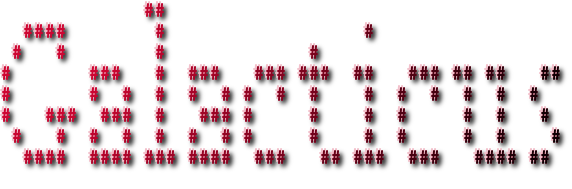
\includegraphics[width=125mm]{GalacticusLogo.png}\\

\Huge Installing and Using \normalsize

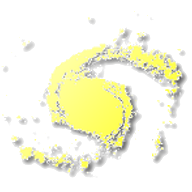
\includegraphics{New_Logo_Galaxy_192_Transparent.png}\\
A semi-analytic galaxy formation code.\\

\copyright\ 2009, 2010 2011, 2012, 2013, 2014, 2015, 2016, 2017, 2018, 2019, 2020 Andrew Benson
\end{center}

\tableofcontents

\mainmatter
\pagestyle{headings}


\chapter{About Galacticus}

\glc\ is a semi-analytic model of galaxy formation. It solves equations describing how galaxies evolve in a merging hierarchy of dark matter halos in a cold dark matter universe. \glc\ has much in common with other semi-analytic models, such as the range of physical processes included and the type of quantities that it can predict.

In designing \glc\ our main goal was to make the code flexible, modular and easily extensible. Much greater priority was placed on making the code easy to use and modify than on making it fast. We believe that a modular and extensible nature is crucial as galaxy formation is an evolving science. In particular, key design features are:
\begin{description}
 \item [Extensible methods for all functions:] Essentially all functions within \glc\ are designed to be extensible, meaning that you can write your own version and insert it into \glc\ easily. For example, suppose you want to use an improved functional form for the \gls{cdm} halo mass function. You would simply write a subroutine conforming to a specified template that computes this mass function and add a short directive (see \S\ref{sec:CodeDirectives}) in your code which explains to the build system how to insert this function in \glc. A recompile of the code will then incorporate your new function.

 \item [Extensible components for tree nodes:] The basic structure in \glc\ is a merger tree, which consists of a linked tree of nodes which have various properties. \glc\ works by evolving the nodes forwards in time subject to a collection of differential equations and other rules. Each node can contains an arbitrary number of \emph{components}. A component may be a dark matter halo, a galactic disk, a black hole etc. Each component may have an arbitrary number of \emph{properties} (some of which may be evolving, others of which can be fixed). \glc\ makes it easy to add additional components. For example, suppose you wanted to add a ``stellar halo'' components (consisting of stars stripped from satellite galaxies). To do this, you would write a module which specifies the following for this component:
 \begin{itemize}
  \item Number of properties;
  \item Interfaces to set and get property values and rates of change;
  \item ``Pipes'' which allow for flows of mass/energy/etc. from one component to another;
  \item Functions describing the differential equations which govern the evolution of the properties;
  \item Functions describing how the component responds to various events (e.g. the node becoming a satellite, a galaxy-galaxy merger, etc.);
  \item Auxiliary functions for handling outputs etc.
 \end{itemize}
 Short directives embedded in this module explain to the \glc\ build system how to incorporate the new component. A recompile will then build your new component into \glc. Typically, a new component can be created quickly by copying an existing one and modifying it as necessary. Furthermore, multiple implementations of a component are allowed. For example, \glc\ contains a component which is a Hernquist spheroid. You could add a de Vaucouler's spheroid component. A simple input parameter then allows you to select which implementation will be used in a given run.

 \item [Centralized ODE solver:] \glc\ evolves nodes in merger trees by calling an ODE solver which integrates forwards in time to solve for the evolution of the properties of each component in a node. This means that you do not need to provide explicit solutions for ODEs (in many cases such solutions are not available anyway) and timestepping is automatically handled to achieve a specified level of precision. The ODE solver allows for the evolution to be interrupted. A component may trigger an interrupt at any time and may do so for a number of reasons. A typical use is to actually create a component within a given node---for example when gas first begins to cool and inflow in a node the disk component must be created. Other uses include interrupting evolution when a merging event occurs.
\end{description}

\subsection{License}

Copyright 2009, 2010, 2011, 2012, 2013, 2014, 2015, 2016, 2017, 2018, Andrew Benson \href{mailto:abenson@carnegiescience.edu}{\normalfont \ttfamily <abenson@carnegiescience.edu>}\\

\glc\ is free software: you can redistribute it and/or modify
it under the terms of the GNU General Public License as published by
the Free Software Foundation, either version 3 of the License, or
(at your option) any later version.

\glc\ is distributed in the hope that it will be useful,
but WITHOUT ANY WARRANTY; without even the implied warranty of
MERCHANTABILITY or FITNESS FOR A PARTICULAR PURPOSE.  See the
GNU General Public License for more details.

You should have received a copy of the GNU General Public License
along with \glc.  If not, see \href{http://www.gnu.org/licenses/}{\normalfont \ttfamily <http://www.gnu.org/licenses/>}.


\chapter{Running Galacticus}

\section{Configuration File}\label{sec:ConfigFile}\index{galacticusConfig.xml@{\tt galacticusConfig.xml}}\index{configuration}

The file {\tt galacticusConfig.xml}, is present, is used to configure \glc\ and provide useful information. It should have the following structure:
\begin{verbatim}
<config>
  <contact>
    <name>My Name</name>
    <email>me@ivory.towers.edu</email>
  </contact>
  <email>
    <host>
      <name>myComputerHostName</name>
      <method>smtp</method>
      <host>smtp-server.ivory.towers.edu</host>
      <user>myUserName</user>
      <passwordFrom>kdewallet</passwordFrom>
    </host>
    <host>
      <name>default</name>
      <method>sendmail</method>
    </host>
  </email>
</config>
\end{verbatim}
The name and e-mail address in the {\tt contact} section will be stored in any \glc\ models run---this helps track the provenance of the model. The {\tt email} section determines how e-mail will be sent. Within this section, you can place one or more {\tt host} elements, the {\tt name} element of which specifies the host name of the computer to which these rules apply (the {\tt default} host is used if no other match is found). For each host, the {\tt method} element specifies how e-mail should be sent, either by {\tt sendmail} or via {\tt smtp}. For SMTP transport (which currently supports SSL connections only), you must specify the {\tt host} SMTP server, {\tt user} name. The {\tt passwordFrom} element specifies how the password for the SMTP log in should be obtained. If set to {\tt input} then the user will be prompted for the password as needed. Alternatively, if you use the \href{http://www.kde.org/}{KDE} desktop and the \href{http://utils.kde.org/projects/kwalletmanager/}{KDEWallet} password manager, setting {\tt passwordFrom} to {\tt kdewallet} will cause the password to be stored in the KDE wallet and retrieved from there subsequently.

\section{Parameter Files}

\glc\ requires a file of parameters to be given as a command line argument. The parameter file is an XML file (which makes it easy to manipulate and construct these files from within many languages, e.g. Perl) with the following structure:
\begin{verbatim}
 <parameters>
   <parameter>
     <name>parameter1name</name>
     <value>parameter1value</value>
   </parameter>
   .
   .
   .
 </parameters>
\end{verbatim}
Each {\tt parameter} element contains {\tt name} and {\tt value} elements which contain the parameter name and desired value respectively. The value can be a number, word(s) or an array of space-separated numbers. Parameters are used to control the values of numerical parameters and also to select methods and other options. If a parameter is not specified in the file a default value (hard coded into \glc) will be used instead. The default values have been chosen to produce a realistic model of galaxy formation, but may change as \glc\ evolves.

All parameter values (both those specified in this file and those set to default) used during a \glc\ run are output to the {\tt Parameters} group within the \glc\ output file. The script {\tt scripts/aux/Extract\_Parameter\_File.pl} will, if given a \glc\ output file, extract the parameters from it and output them into an XML file suitable for re-input into \glc.

\subsection{Generating Parameter Files}\index{parameters!generating}

Some scripts are provided which assist in the generation of parameter files. These are located in the {\tt scripts/parameters/} folder and are detailed below:
\begin{description}
\item [{\tt cosmologicalParametersMonteCarlo.pl}] This script will generate a set of cosmological parameters drawn at random from the WMAP-7 constraints \cite{komatsu_seven-year_2010}. It uses the covariance matrix (currently defined in {\tt data/Cosmological\_Parameters\_WMAP-7.xml}) to produce correlated random variables\footnote{Note that this does not capture the full details of the correlations between parameters, since it uses just the covariance matrix. For a more accurate calculation the full Monte Carlo Markov Chains used in the WMAP-7 parameter fitting should be used instead.}. The generated parameters are printed to standard output as \glc-compatible XML.
\end{description}

\section{Running Galacticus}

\glc\ is running using
\begin{verbatim}
 Galacticus.exe [<parameterFile>]
\end{verbatim}
where {\tt parameterFile} is the name of the file containing a list of parameter values for \glc. \glc\ will display messages indicating its progress as it runs (the verbosity can be controlled with the {\tt verbosityLevel} parameter).

\subsection{Restarting A Crashed Run}\label{sec:Restarting}

If \glc\ crashes, it can be useful to restart the calculation from just prior to the crash to speed the debugging process. \glc\ has functionality to store and retrieve the internal state of any modules and to recover this to permit such restarting. Currently, this is implemented with the {\tt build} method of merger tree construction, such that the internal state is stored prior to commencing the building of each tree, thereby allowing a calculation to be restarted with the tree that crashed. More general store/retrieve behavior is planned for future releases.

To cause \glc\ to periodically store its internal state include the following input parameter:
\begin{verbatim}
  <parameter>
    <name>stateFileRoot</name>
    <value>galacticusState</value>
  </parameter>
\end{verbatim}
This will cause the internal state to be stored to files {\tt galacticusState.state} and {\tt galacticusState.fgsl.state} prior to commencing building each merger tree. Should a tree crash then replace this input parameter with:
\begin{verbatim}
  <parameter>
    <name>stateRetrieveFileRoot</name>
    <value>galacticusState</value>
  </parameter>
  <parameter>
    <name>mergerTreeBuildTreesBeginAtTree</name>
    <value>N</value>
  </parameter>
\end{verbatim}
where {\tt N} is the number of the tree that crashed. This will cause calculations to begin with tree {\tt N} and for the internal state to be recovered from the above mentioned files. The resulting tree and all galaxy formation calculations should therefore proceed just as in the original run (and so create the same crash condition).

\subsection{Running Grids of Models}\label{sec:RunningGrids}

You can easily write your own scripts to generate parameter files and run \glc\ on these files. An example of such a script is {\tt scripts/aux/Run\_Galacticus.pl}. This script will loop over a sequence of parameter values, generate appropriate parameter files, run \glc\ using those parameters and analyze the results. This script currently supports running of \glc\ on a local machine or on a \href{http://www.cs.wisc.edu/condor/}{{\sc Condor}}\index{Condor} cluster. To run the script simply enter:
\begin{verbatim}
 ./scripts/aux/Run_Galacticus.pl <runFile>
\end{verbatim}
This will launch a single instance of the script. Multiple instances can be launched and will share the work load (i.e. they will not attempt to run a model which another instance is already running or has finished). If multiple instances are to be launched on multiple machines a command line option to {\tt Run\_Galacticus.pl} can be used to ensure that they do not duplicate work. Adding {\tt --instance 2:4} for example will tell the script to run only the second model from each block of four models it finds. Launching for {\tt Run\_Galacticus.pl} scripts on four different machines with {\tt --instance 1:4}, {\tt --instance 2:4}, {\tt --instance 3:4} and {\tt --instance 4:4} will then divide the models between those machines.

The {\tt runFile} is an XML file with the following structure:
\begin{verbatim}
<parameterGrid>
 <modelRootDirectory>models.new</modelRootDirectory>
 <baseParameters>newBestParametersQuick.xml</baseParameters>
 <threadCount>maximum</threadCount>
 <condor>
   <useCondor>true</useCondor>
   <galacticusDirectory>/home/condor/Galacticus/v0.9.0</galacticusDirectory>
   <universe>vanilla</universe>
   <environment>LD_LIBRARY_PATH=/usr/lib:/usr/lib64:/usr/local/lib</environment>
   <requirement>Memory &gt;= 1000 &amp;&amp; Memory &lt; 2000</requirement>
 </condor>
 <parameters>
  <label>modelLabel</label>
  <parameter>
   <name>stabilityThresholdStellar</name>
   <value>1.1</value>
   <value>0.9</value>
  </parameter>
 </parameters>
 <parameters>
  <parameter>
   <name>stabilityThresholdGaseous</name>
   <value>1.1</value>
   <value>0.9</value>
  </parameter>
  <parameter>
   <name>imfSalpeterYieldInstantaneous</name>
   <value>0.02</value>
   <value>0.04</value>
  </parameter>
  <parameter>
   <name>starFormationTimescaleDisksMethod</name>
   <value>Kennicutt-Schmidt
    <parameter>
     <name>starFormationKennicuttSchmidtTruncate</name>
     <value>true</value>
     <value>false</value>
    </parameter>
   </value>
   <value>dynamical time</value>
  </parameter>
 </parameters>
</parameterGrid>
\end{verbatim}
Each {\tt parameters} block contains a list of parameters following the format used in standard \glc\ parameter files, with the difference that each parameter can have multiple {\tt values}. A model will be run for all possible combinations of these values. Additionally, any {\tt value} element may contain further {\tt parameter} elements. All possible values of these parameters will be looped over when, and only when, the appropriate value of the containing parameter is being used. For example, in the above example, models will be run with {\tt [starFormationKennicuttSchmidtTruncate]}$=${\tt true} and {\tt false} only when {\tt [starFormationTimescaleDisksMethod]}$=${\tt Kennicutt-Schmidt} and not when {\tt [starFormationTimescaleDisksMethod]}$=${\tt dynamical time}.

By default, each model is output into a sequentially numbered directory within the {\tt ./models} directory. By default, these directories have the prefix {\tt galacticus}. This can be changed by including a {\tt label} element inside a {\tt parameters} block, in which case the content of the {\tt label} element will be used as the prefix. This root directory can be modfified by the optional {\tt modelRootDirectory} element. Additionally, a set of base parameters can be read from a file specified by the {\tt baseParameters} file---these will be read before each model is run and before any variations in parameters for the specific model are applied. As such, it defines the default model around which parameter variations occur. Additional options that may be present in the file (as elements within the {\tt parameterGrid} element) are:
\begin{description}
\item[{\tt doAnalysis}]If set to ``no'' then no analysis scripts will be run on completed models, otherwise, they will be. Optionally, the analysis script to run can be specified via the {\tt analysisScript} element (see \S\ref{sec:AnalysisScripts});
\item[{\tt emailReport}] If set to ``yes'' a report will be e-mailed to the address specified in {\tt galacticusOptions.xml} when a model fails. Otherwise, the report will be written to standard output instead.
\item[{\tt threadCount}] Specifies the number of threads that should be launched (each running a separate \glc\ model) when running on the local machine. If set to ``maximum'' then the number of threads will be set to the available number of cores on the local machine. If not present, a single thread is used.
\item[{\tt condor}] This section, if present, specifies if and how jobs should be submitted to a {\tt Condor} cluster. The following options are available:
\begin{description}
\item[{\tt useCondor}] If set to ``true'' then jobs will be submitted to a {\sc Condor} cluster, otherwise they will be run on the local machine;
\item[{\tt galacticusDirectory}] When a \glc\ job is submitted to a {\sc Condor} cluster the \glc\ executable and the input parameter file are transferred to the machine where the job runs. Other files, such as data files, are not transferred. Therefore, they must be already present on any remote machine on which the job can run. This option specifies where a complete \glc\ installation can be found on the remote machine. If not present, it defaults to {\tt /home/condor/Galacticus/v0.9.0};
\item[{\tt universe}] Specifies to which {\sc Condor} universe jobs should be submitted. Allowed options are ``vanilla'' and ``standard''. If the standard universe is to be used then \glc\ must have been linked with {\tt condor\_compile}---the {\tt Makefile} allows this if the relevant lines are uncommented;
\item[{\tt environment}] Any settings here are passed to {\sc Condor}'s {\tt environment} option in order to set appropriate environment variables on the machine where a job is executed;
\item[{\tt requirement}] Any setting here is passed to {\sc Condor}'s {\tt requirements} option to specify requirements for each job. Multiple {\tt requirement} entries will be combined (using logical and).
\end{description}
\end{description}

In addition to the {\tt galacticus.hdf5} output file, each model directory will contain a file {\tt newParameters.xml} which contains the parameters used to run the model and {\tt galacticus.log} which contains any output from \glc\ during the run.

If present, the file {\tt galacticusConfig.xml}, described in \S\ref{sec:ConfigFile}, is parsed for configuration options. If the {\tt contact} element is present, the listed name and e-mail address will be used to determine who should receive error reports should a model crash. The error report will contain the host name of the computer running the model, the location of the model output and the log file (which may be incomplete if output is being buffered). Additionally, any core file produced will be stored in the model directory for later perusal, and the state files (see \S\ref{sec:Restarting}) for the run can also be found in the model directory.

\subsection{Analysis of Models}\label{sec:AnalysisScripts}

The {\tt Run\_Galacticus.pl} script will automatically run {\tt scripts/analysis/Galacticus\_Compute\_Fit.pl} on each model to generate plots and fitting data unless {\tt doAnalysis}$=${\tt no} is set in the {\tt runFile} (see \S\ref{sec:RunningGrids}). This script, which can also be running manually using
\begin{verbatim}
 ./scripts/analysis/Galacticus_Compute_Fit.pl <galacticusFile> <outputDirectory> [<analysisFile>]
\end{verbatim}
where {\tt galacticusFile} is the name of the \glc\ output file to analyze and {\tt outputDirectory} is the directory into which plots and fitting data should be placed, reads the file {\tt \textless analysisFile\textgreater} (or {\tt data/Galacticus\_Compute\_Fit\_Analyses.xml} if {\tt \textless analysisFile\textgreater} is not specified) which has the following structure:
\begin{verbatim}
 <analyses>
  <analysis>
    <script>scripts/plotting/Plot_HI_Mass_Function.pl</script>
    <weight>1.0</weight>
  </analysis>
  <analysis>
    <script>scripts/plotting/Plot_K_Luminosity_Function.pl</script>
    <weight>1.0</weight>
  </analysis>
  .
  .
  .
 </analyses>
\end{verbatim}
Each {\tt analysis} element contains the name of a script to run to perform some analysis and a weight to be given to the results of this analysis when combining results to get a net goodness of fit. Each script listed will be run and is expected to have accept arguments of the form:
\begin{verbatim}
 My_Analysis_Script.pl <galacticusFile> <outputDirectory> <showFit>
\end{verbatim}
where the {\tt showFit} argument can be 0 or 1 and, if set to 1, the script should output an XML chunk to standard output giving details of its fitting analysis. This chunk should have the form:
\begin{verbatim}
 <galacticusFit>
   <name>Description of this analysis</name>
   <chiSquared>24.5</chiSquared>
   <degreesOfFreedom>19</degreesOfFreedom>
   <fileName>Output_File_Name.pdf</fileName>
 </galacticusFit>
\end{verbatim}
where {\tt chiSquared} and {\tt degreesOfFreedom} are the fitting results. All such data returned from fitting scripts will be collated by {\tt Galacticus\_Compute\_Fit.pl}, augmented with the weight value and the net goodness of fit determined. All of this information is then output to {\tt galacticusFits.xml} in the selected output directory.

\subsection{Running Models in ``Embarrassingly Parallel'' Mode}

While \glc\ is parallelized via OpenMP it is also possible to split a given model across several ``worker'' CPUs on one or more computers. The trees to be processed will be shared between these workers and the results can be later recombined. To use this ``poor man's'' parallelization, add the following to a model parameter file:
\begin{verbatim}
  <parameter>
    <name>treeEvolveWorkerCount</name>
    <value>N</value>
  </parameter>
  <parameter>
    <name>treeEvolveWorkerNumber</name>
    <value>i</value>
  </parameter>
\end{verbatim}
where {\tt N} is the total number of workers to be used and {\tt i} is the number of this worker (ranging from 1 to {\tt N}). Once all workers have finished, their outputs can (if required) be combined into a single output file using the {\tt Merge\_Models.pl} script as follows:
\begin{verbatim}
./scripts/aux/Merge_Models.pl <model1> <model2> .... <modelOutput>
\end{verbatim}
where {\tt model1} etc. are the names of the various output files and {\tt modelOutput} is the file into which the combined results should be placed. The {\tt Merge\_Models.pl} script will combine all merger trees into the output file and will additionally cumulate any data in the {\tt globalHistory} groups in these files. The UUIDs of the merged files (see \S\ref{sec:UUID}) will be concatenated (with a ``:'' separator) and placed into the {\tt UUIDs} attribute of the new file. Additionally, a new UUID will be generated and stored in the {\tt UUID} attribute of the new file.

\section{Additional Codes}

The \glc\ code base can be used for other calculations. Some examples of such usage (and which are sufficiently useful in their own right) are included and are detailed in this section.

\subsection{{\tt Halo\_Mass\_Functions}}

The {\tt Halo\_Mass\_Functions} code will generate an HDF5 output file which contains a variety of measures of the dark matter halo mass function tabulated as a function of mass and at a variety of redshifts. The code is built and run as follows:
\begin{verbatim}
make Halo_Mass_Functions.exe
Halo_Mass_Functions.exe <parameterFile> <outputFile>
\end{verbatim}
where {\tt parameterFile} is a file of parameters in \glc's usual XML format and {\tt outputFile} is the name of the file to which the halo mass function data will be written. The parameter file can specify any parameters needed for computing the mass function (they will be set to default values in cases where a paramter is not included). The redshifts at which to output halo mass functions are given by the {\tt [outputRedshifts]} parameter. In addition to the usual \glc\ parameters three additional parameters control behavior:
\begin{description}
\item [{\tt [haloMassFunctionsMassMinimum]}] The lowest mass halo (in units of $M_\odot$) at which to tabulate;
\item [{\tt [haloMassFunctionsMassMaximum]}] The highest mass halo (in units of $M_\odot$) at which to tabulate;
\item [{\tt [haloMassFunctionsPointsPerDecade]}] The number of points per decade of halo mass at which to tabulate.
\end{description}
The output file has the following structure:
\begin{verbatim}
+-> Outputs
|   |
|   +-> outputCharacteristicMass      [dataset]
|   |
|   +-> outputCriticalOverdensities   [dataset]
|   |
|   +-> outputExpansionFactor         [dataset]
|   |
|   +-> outputGrowthFactors           [dataset]
|   |
|   +-> outputRedshift                [dataset]
|   |
|   +-> outputTime                    [dataset]
|   |
|   +-> outputVirialDensityContrast   [dataset]
|    
+-> Parameters
|   |
|   +-> parameter1                    [attribute]
|   |
|   +-> parameterN                    [attribute]
|    
+-> haloMassFunctions
    |
    +-> haloBias                      [dataset]
    |
    +-> haloMass                      [dataset]
    |
    +-> haloMassFractionCumulative    [dataset]
    |
    +-> haloMassFunctionCumulative    [dataset]
    |
    +-> haloMassFunctionLnM           [dataset]
    |
    +-> haloMassFunctionM             [dataset]
    |
    +-> haloNu                        [dataset]
    |
    +-> haloSigma                     [dataset]
    |
    +-> haloVirialRadius              [dataset]
    |
    +-> haloVirialTemperature         [dataset]
    |
    +-> haloVirialVelocity            [dataset]
\end{verbatim}
The {\tt Parameters} group contains attributes giving the values of all used parameters (just as in a \glc\ output file). The {\tt Outputs} group contains datasets which give global properties at each requested output time as follows:
\begin{description}
\item [{\tt outputCharacteristicMass}] The characteristic mass scale (in units of $M_\odot$), $M_*$, at which $\sigma(M)=\delta_{\rm c}(z)$;
\item [{\tt outputCriticalOverdensities}] The critical overdensity for collapse of halos, $\delta_{\rm c}$;
\item [{\tt outputExpansionFactor}] The expansion factor;
\item [{\tt outputGrowthFactors}] The linear growth factor;
\item [{\tt outputRedshift}] The redshift;
\item [{\tt outputTime}] The cosmic time (in units of Gyr);
\item [{\tt outputVirialDensityContrast}] The virial density contrast of halos.
\end{description}
The {\tt haloMassFunctions} group contains datasets which list the properties of halos as a function of mass at each requested output time as follows:
\begin{description}
\item [{\tt haloBias}] The large scale linear theory bias of the halo;
\item [{\tt haloMass}] The mass of the halo (in $M_\odot$);
\item [{\tt haloMassFractionCumulative}] The mass fraction in halos above the current halo mass;
\item [{\tt haloMassFunctionCumulative}] The cumulative number of halos per unit volume above the current halo mass (in units of Mpc$^{-3}$);
\item [{\tt haloMassFunctionLnM}] The halo mass function per logarithmic halo mass (in units of Mpc$^{-3}$);
\item [{\tt haloMassFunctionM}] The halo mass function per logarithmic halo mass (in units of Mpc$^{-3} M_\odot^{-1}$);
\item [{\tt haloNu}] The peak height of the halo, $\nu = \delta_{\rm c}/\sigma(M)$;
\item [{\tt haloSigma}] The root-variance of the mass field smoothed in top-hat spheres;
\item [{\tt haloVirialRadius}] The virial radius (in units of Mpc) of the current halo mass;
\item [{\tt haloVirialTemperature}] The virial temperature (in units of Kelvin) of the current halo mass;
\item [{\tt haloVirialVelocity}] The virial velocity (in units of km/s) of the current halo mass;
\end{description}
Dimensionful datasets have an {\tt unitsInSI} attribute that gives their units in the SI system.

\subsection{{\tt Power\_Spectra}}\index{power spectrum!outputting}

The {\tt Power\_Spectra} code will generate an HDF5 output file which contains a variety of measures of the matter power spectrum tabulated as a function of wavenumber. The code is built and run as follows:
\begin{verbatim}
make Power_Spectra.exe
Power_Spectra.exe <parameterFile> <outputFile>
\end{verbatim}
where {\tt parameterFile} is a file of parameters in \glc's usual XML format and {\tt outputFile} is the name of the file to which the power spectrum data will be written. The parameter file can specify any parameters needed for computing the power spectrum (they will be set to default values in cases where a parameter is not included).
The output file has the following structure:
\begin{verbatim}
+-> powerSpectrum
|   |
|   +-> alpha         [dataset]
|   |
|   +-> mass          [dataset]
|   |
|   +-> powerSpectrum [dataset]
|   |
|   +-> sigma         [dataset]
|   |
|   +-> wavenumber    [dataset]
|    
+-> Parameters
    |
    +-> parameter1    [attribute]
    |
    +-> parameterN    [attribute]
\end{verbatim}
The {\tt Parameters} group contains attributes giving the values of all used parameters (just as in a \glc\ output file). The {\tt powerSpectrum} group contains datasets which give the power spectrum and related properties as follows:
\begin{description}
\item [{\tt alpha}] The logarithmic slope of $\sigma(M)$: $\alpha = {\rm d} \ln \sigma / {\rm d} \ln M$;
\item [{\tt mass}] The mass scale, $M$, corresponding to the given wavenumber, $k$, defined such that $M=4 \pi \Omega_0 \rho_{\rm crit} / 3 k^3$ (in units of $M_\odot$);
\item [{\tt powerSpectrum}] The linear theory power spectrum at $z=0$: $P(k)$ in units of Mpc$^3$;
\item [{\tt sigma}] The dimensionless linear theory mass fluctuation at $z=0$: $\sigma(M)$;
\item [{\tt wavenumber}] The wavenumber in units of Mpc$^{-1}$.
\end{description}
Dimensionful datasets have an {\tt unitsInSI} attribute that gives their units in the SI system.


\chapter{Input Data}

In some configurations, \glc\ requires additional input data to run. For example, if asked to process galaxy formation through a set of externally derived merger trees, then a file describing those trees must be given. In the remainder of this section we describe the structure of external datasets which can be inputs to \glc.

\section{Broadband Filters}\index{filters!broadband}

To compute luminosities through a given filter, \glc\ requires the response function, $R(\lambda)$, of that filter to be defined. \glc\ follows the convention of \cite{hogg_k_2002} in defining the filter response to be the fraction of incident photons received by the detector at a given wavelength, multiplied by the relative photon response (which will be 1 for a photon-counting detector such as a CCD, or proportional to the photon energy for a bolometer/calorimeter type detector. Filter response files are stored in {\normalfont \ttfamily data/filters/}. Their structure is shown below, with the {\normalfont \ttfamily SDSS\_g.xml} filter reponse file used as an example:
\begin{verbatim}
 <filter>
  <description>SDSS g vacuum (filter+CCD +0 air mass)</description>
  <name>SDSS g</name>
  <origin>Michael Blanton</origin>
  <response>
    <datum>   3630.000      0.0000000E+00</datum>
    <datum>   3680.000      2.2690000E-03</datum>
    <datum>   3730.000      5.4120002E-03</datum>
    <datum>   3780.000      9.8719997E-03</datum>
    <datum>   3830.000      2.9449999E-02</datum>
    .
    .
    . 
  </response>
  <effectiveWavelength>4727.02994472695</effectiveWavelength>
  <vegaOffset>0.107430167298754</vegaOffset>
</filter>
\end{verbatim}
The {\normalfont \ttfamily description} tag should provide a description of the filter, while the {\normalfont \ttfamily name} tag provides a shorter name. The {\normalfont \ttfamily origin} tag should describe from where/whom this filter originated. The {\normalfont \ttfamily response} element contains a list of {\normalfont \ttfamily datum} tags each giving a wavelength (in Angstroms) and response pair. The normalization of the response is arbitrary. The {\normalfont \ttfamily effectiveWavelength} tag gives the mean, response-weighted wavelength of the filter and is used, for example, in dust attenuation calculations. The {\normalfont \ttfamily vegaOffset} tag gives the value (in magnitudes) which must be added to an AB-system magnitude in this system to place it into the Vega system. Both {\normalfont \ttfamily effectiveWavelength} and {\normalfont \ttfamily vegaOffset} can be computed by running
\begin{verbatim}
 scripts/filters/vega_offset_effective_lambda.pl data/filters
\end{verbatim}
which will compute these values for any filter files that do not already contain them and append them to the files.

\section{Merger Trees}\label{sec:MergerTreeFiles}

While \glc\ can build merger trees using analytic methods it is often useful to be able to utilize merger trees from other sources (e.g. extracted from an N-body simulation). To facilitate this, \glc\ allows merger trees to be read from an HDF5 file\footnote{The following assumes that merger trees will be read from a file following \protect\glc's standard HDF5 format which is described in \S\protect\ref{sec:MergerTreeFileFormat}. Other formats can also be read by selecting the relevant importer via the {\normalfont \ttfamily [mergerTreeImporterMethod]} parameter.}. To do so, set the {\normalfont \ttfamily [mergerTreeConstructMethod]} input parameter to {\normalfont \ttfamily read} and specify the filename to read via their {\normalfont \ttfamily [mergerTreeReadFileName]} parameter.

The HDF5 file should follow the general purpose format described in \S\ref{sec:MergerTreeFileFormat}. An example of how to construct such a file can be found in the {\normalfont \ttfamily tests/nBodyMergerTrees} folder. In that folder, the {\normalfont \ttfamily getMillenniumTrees.pl} script will retrieve a sample of merger trees from the \href{http://www.g-vo.org/MyMillennium3/}{Millennium Simulation database} and use the {\normalfont \ttfamily Merger\_Tree\_File\_Maker.exe} code supplied with \glc\ to convert these into an HDF5 file suitable for reading into \glc. The {\normalfont \ttfamily getMillenniumTrees.pl} script requires you to have a username and password to access the Millennium Simulation database\footnote{If you do not have a username and password for the Millennium Simulation database you can request one from \href{mailto:contact@g-vo.org}{\normalfont \ttfamily contact@g-vo.org}.}. These can be entered manually or stored in a section of the {\normalfont \ttfamily galacticusConfig.xml} file (see \S\ref{sec:ConfigFile}) as follows:
\begin{verbatim}
  <millenniumDB>
    <host>
      <name>^myHost$</name>
      <user>myUserName</user>
      <passwordFrom>input</passwordFrom>
      <treePath>/path/to/trees</treePath>
    </host>
    <host>
      <name>default</name>
      <user>myUserName</user>
      <password>myPassword</password>
    </host>
  </millenniumDB>
\end{verbatim}
Here, each {\normalfont \ttfamily host} section describes rules for a given computer (with ``default'' being used if no specific match to the regular expression give in {\normalfont \ttfamily name} is found). The {\normalfont \ttfamily user} element gives the user name to use, while the {\normalfont \ttfamily passwordFrom} element specifies how the password should be obtained. Currently the only allowed mechanism is ``input'', in which case the password is read from standard input. Alternatively, you can include a {\normalfont \ttfamily password} element which contains the password itself. Of course, this is insecure\ldots

The optional {\normalfont \ttfamily treePath} element gives the location where merger trees from the Millennium Simulation can be stored. Some scripts will make use of this location so that Millennium Simulation merger trees can be shared between multiple scripts.

\subsection{Processing of Merger Tree Files}\label{sec:MergerTreeFileProcessing}

The ``read'' merger tree construction method (see \S\ref{sec:MergerTreeConstruction}) reads these files and processes them into a form suitable for \glc\ to evolve. Merger trees are inherently complex structures, particularly when the possibility of subhalos are considered. \glc\ is currently designed to work with single descendent merger trees, i.e. ones in which the tree structure is entirely defined by specifying which \gls{node} a given \gls{node} is physically associated with at a later time. Additionally, \glc\ expects the merger tree file to contain information on the host \gls{node}, i.e. the node within which a given node is physically located. In the following, these two properties are labelled {\normalfont \ttfamily descendentNode} and {\normalfont \ttfamily hostNode}. \glc\ assumes that nodes for which {\normalfont \ttfamily descendentNode}$=${\normalfont \ttfamily hostNode} are isolated halos (i.e. they are their own hosts) while other nodes are subhalos (i.e. they are hosted by some other node). An example of a simple tree structure is shown in Fig.~\ref{fig:MergerTreeSimple}. The particular structure would be represented by the following list of nodes and node properties (a $-1$ indicates that no descendent node exists):
\begin{center}
\begin{tabular}{rrr}
\hline
{\normalfont \ttfamily node} & {\normalfont \ttfamily descendentNode} & {\normalfont \ttfamily hostNode} \\
\hline
1 & -1 & 1 \\
2 &  1 & 2 \\
3 &  2 & 3 \\
4 &  1 & 4 \\
5 &  4 & 5 \\
6 & -1 & 1 \\
7 &  6 & 4 \\
8 &  7 & 8 \\
\hline
\end{tabular}
\end{center}

\begin{figure}
 \begin{center}
 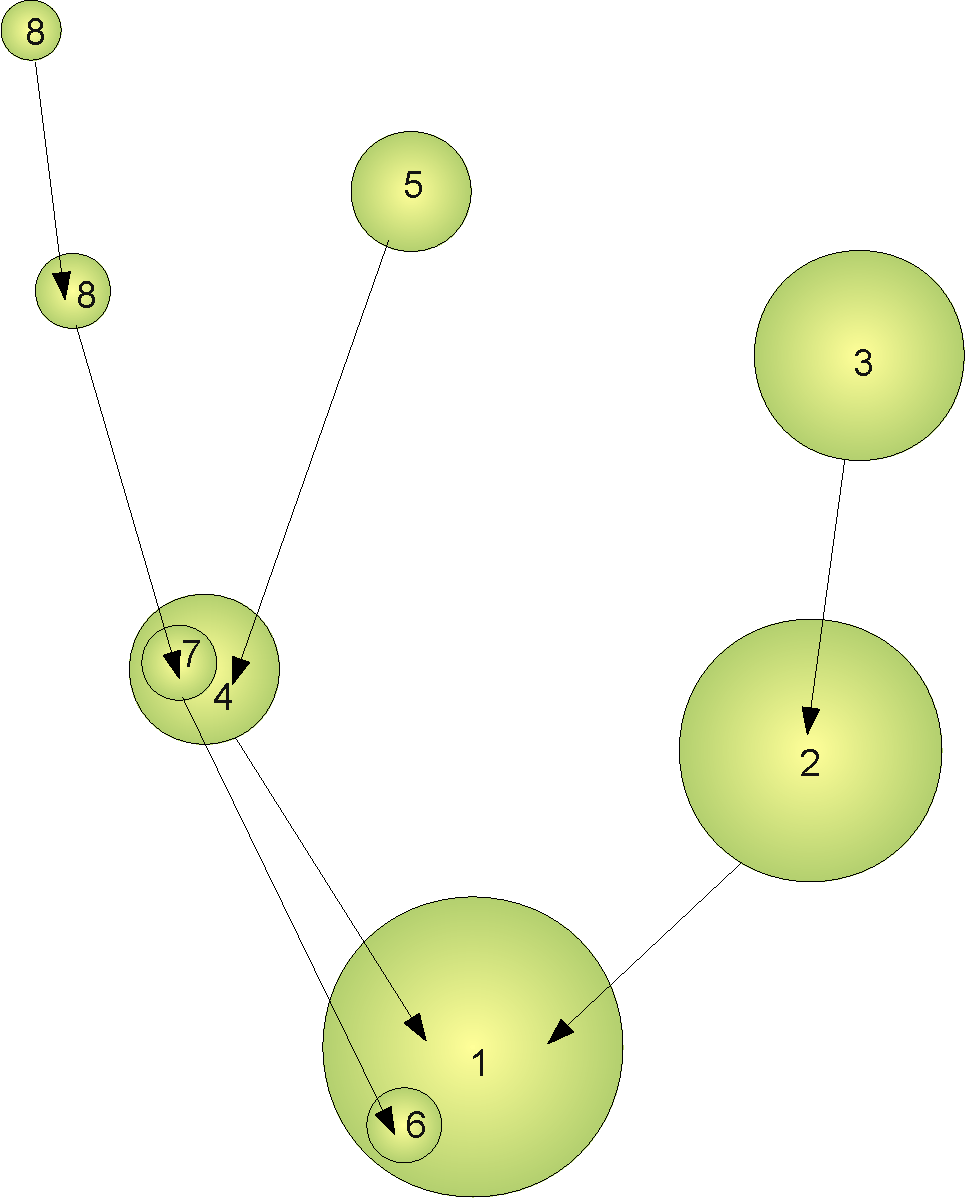
\includegraphics[width=160mm]{Diagrams/MergerTreeSimple.pdf}
 \end{center}
 \caption{An example of a simple merger tree structure. Colored circles represent nodes in the merger tree. Each node has a unique index indicated by the number inside each circle. Black arrows link each node to its descendent node (as specified by the {\normalfont \ttfamily descendentNode} property. Where a node is not its own host node it is placed inside its host node.}
 \label{fig:MergerTreeSimple}
\end{figure}

The following should be noted when constructing merger tree files:
\begin{itemize}
\item Note that \glc\ does not require that nodes be placed on a uniform grid of times/redshifts, nor that mass be conserved along a branch of the tree. After processing the tree in this way, \glc\ builds additional links which identify the child node of each halo and any sibling nodes. These are not required to specify the tree structure but are computationally convenient.
\item It is acceptable for a node to begin its existence as a subhalo (i.e. to have never had an isolated node progenitor). Such nodes will be created as satellites in the merger tree and, providing the selected node components (see \S\ref{sec:Components}) initialize their properties appropriately, will be evolved correctly.
\item It is acceptable for an isolated node to have progenitors, none of which are a primary progenitor. This can happen if all progenitors descend into subhalos in the isolated node. In such cases, \glc\ will create a clone of the isolated node at a very slightly earlier time to act as the primary progenitor. This is necessary to allow the tree to be processed correctly, but does not affect the evolution of the tree.
\item Normally, cases where a node's host node cannot be found in the \gls{forest} will cause \glc\ to exit with an error. Setting {\normalfont \ttfamily [mergerTreeReadMissingHostsAreFatal]}$=${\normalfont \ttfamily false} will instead circumvent this issue by making any such nodes self-hosting (i.e. they become isolated nodes rather than subhalos). Note that this behavior is not a physically correct way to treat such cases---it is intended only to allow trees to be processed in cases where the full \gls{forest} is not available.
\item It is acceptable for nodes to jump between branches in a tree, or even to jump between branches in different trees. In the latter case, all trees linked by jumping nodes (a so-called ``\gls{forest}'' of connected trees) must be stored as a single forest (with multiple root-nodes) in the merger tree file. \glc\ will process this \gls{forest} of trees simultaneously, allowing to nodes to move between their branches.
\item It is acceptable for a subhalo to later become an isolated halo (as can happen due to three-body interactions; see  \citealt{sales_cosmic_2007}). If {\normalfont \ttfamily [mergerTreeReadAllowSubhaloPromotions]}$=${\normalfont \ttfamily true} then such cases will be handled correctly (i.e. the subhalo will be promoted back to being an isolated halo). If {\normalfont \ttfamily [mergerTreeReadAllowSubhaloPromotions]}$=${\normalfont \ttfamily false} then subhalos are not permitted to become isolated halos. In this case, the following logic will be applied to remove all such cases from the tree:\\

\noindent\hspace{ 5mm} $\rightarrow$ \parbox[t]{150mm}{For any branch in a tree which at some point is a subhalo:}\\

\noindent\hspace{10mm} $\rightarrow$ \parbox[t]{145mm}{Beginning from the earliest node in the branch that is a subhalo, repeatedly step to the next descendent node;}\\

\noindent\hspace{10mm} $\rightarrow$ \parbox[t]{145mm}{If that descendent is \emph{not} a subhalo then:}\\

\noindent\hspace{15mm} $\rightarrow$ \parbox[t]{140mm}{If there is not currently any non-subhalo node which has the present node as its descendent then current node is only descendent of a subhalo. Therefore, try to make this node a subhalo, and propose the descendent of the host node of the previous node visited in the branch as the new host:}\\

\noindent\hspace{20mm} $\rightarrow$ \parbox[t]{135mm}{If the proposed host exists:}\\

\noindent\hspace{25mm} $\rightarrow$ \parbox[t]{130mm}{If the mass of the current node is less than that of the proposed host:}\\

\noindent\hspace{30mm} $\rightarrow$ \parbox[t]{125mm}{If the proposed hosts exists before the current node, repeatedly step to its descendents until one is found which exists at or after the time of the current node. This is the new proposed host.}\\

\noindent\hspace{30mm} $\rightarrow$ \parbox[t]{125mm}{If the proposed host is a subhalo, make it an isolated node.}\\

\noindent\hspace{30mm} $\rightarrow$ \parbox[t]{125mm}{The current node is made a subhalo within the proposed host.}\\

\noindent\hspace{25mm} $\rightarrow$ \parbox[t]{130mm}{Otherwise:}\\

\noindent\hspace{30mm} $\rightarrow$ \parbox[t]{125mm}{The current node remains an isolated node, while the proposed host is instead made a subhalo within the current node.}\\

\noindent\hspace{20mm} $\rightarrow$ \parbox[t]{135mm}{Otherwise:}\\

\noindent\hspace{25mm} $\rightarrow$ \parbox[t]{130mm}{The proposed host does not exists, which implies the end of a branch has been reached. Therefore, flag the current node as being a subhalo with a host identical to that of the node from which it descended.}\\
\end{itemize}

\subsubsection{Requirements for \glc\ Input Parameters}

The following requirements must be met for the input parameters to \glc\ when using merger trees read from file:
\begin{itemize}
 \item The cosmological parameters ($\Omega_\mathrm{M}$, $\Omega_\Lambda$, $\Omega_\mathrm{b}$, $H_0$, $\sigma_8$), if defined in the file, must be set identically in the \glc\ input file unless you set {\normalfont \ttfamily [mergerTreeReadMismatchIsFatal]}$=${\normalfont \ttfamily false} in which case you'll just be warned about any mismatch;
 \item \glc\ assumes by default that all merger trees exist at the final output time---if this is not the case set {\normalfont \ttfamily [allTreesExistAtFinalTime]}$=${\normalfont \ttfamily false}.
\end{itemize}

\subsection{Setting of Halo Properties}

\subsubsection{Dark Matter Scale Radii}\index{dark matter halo!concentration}\index{dark matter halo!scale radius}

If {\normalfont \ttfamily [mergerTreeReadPresetScaleRadii]}$=${\normalfont \ttfamily true} and the {\normalfont \ttfamily halfMassRadius} dataset is available within the {\normalfont \ttfamily haloTrees} group (see \S\ref{sec:ForestHalosGroup}) then the half-mass radii of nodes will be used to compute the corresponding scale length of the dark matter halo profile\footnote{The scale radius is found by seeking a value which gives the correct half mass radius. It is therefore important that the definition of halo mass (specifically the virial overdensity) in \protect\glc\ be the same as was used in computing the input half mass radii.}. This requires a dark matter profile scale component which supports setting of the scale length (see \S\ref{sec:DarkMatterProfileComponent}).

\subsubsection{Satellite Merger Times}\index{merger times}\index{satellite!merger times}

If {\normalfont \ttfamily [mergerTreeReadPresetMergerTimes]}$=${\normalfont \ttfamily true} then merger times for satellites will be computed directly from the merger tree data read from file. When a subhalo has an isolated halo as a descendent it is assumed to undergo a merger with that isolated halo at that time. Note that this requires a satellite orbit component method which supports setting of merger times (e.g. {\normalfont \ttfamily [treeNodeMethodSatelliteOrbit]}$=${\normalfont \ttfamily preset}).

\subsubsection{Dark Matter Halo Spins}\index{dark matter halo!spin}

If {\normalfont \ttfamily [mergerTreeReadPresetSpins]}$=${\normalfont \ttfamily true} and the {\normalfont \ttfamily angularMomentum} dataset is available within the {\normalfont \ttfamily haloTrees} group (see \S\ref{sec:ForestHalosGroup}) then the spin parameters of nodes will be computed and set. This requires a dark matter halo spin component which supports setting of the spin (see \S\ref{sec:DarkMatterHaloSpinComponent}).


\chapter{Advanced Usage}

In this chapter we cover in more detail several aspects of \glc, including the structure of parameter files, the strucure of output files, and how to perform various types of analysis.

\section{Parameter Files}\label{sec:ParameterFiles}

As described above, \glc\ requires a file of parameters to be given as a command line argument. The parameter file is an \gls{xml} file (which makes it easy to manipulate and construct these files from within many languages, e.g. Python) with the following structure:
\begin{verbatim}
 <parameters>
   <version>0.9.4</version>
   <formatVersion>2</formatVersion>
   <parameter1Name value= "parameter1Value" />
   <parameter2Name>
     <value>parameter2Value</value>
   </parameter2Name>
   <parameter3Name value= "parameter3Value" >
      <subParameter1Name value= "subParameter1Value" />
      <subParameter2Name value= "subParameter2Value" />
      .
      .
      .
   </parameter3Name>
   .
   .
   .
   <parameter4Name value= "parameter4Value" id="myRefParam" >
      <subParameter1Name value= "subParameter1Value" />
      <subParameter2Name value= "subParameter2Value" />
      .
      .
      .
   </parameter3Name>
   .
   .
   .
   <parameter4Name idRef="myRefParam"/>
   .
   .
   .
   <parameter5Name value="=10.0*[parameter4Name::subParameter1Name]"/>
 </parameters>
\end{verbatim}
Each named element must have a {\normalfont \ttfamily value} attribute (preferred), or else contains a value element, which contains the desired value. The value can be a number, word or an array of space-separated numbers or words. Parameters are used to control the values of numerical parameters and also to select methods and other options. In many cases, if a parameter is not specified in the file a default value (hard coded into \glc) will be used instead. The default values have been chosen to produce a realistic model of galaxy formation, but may change as \glc\ evolves. Parameters may have sub-parameters embedded within them, as in the example above.

Sub-parameters are used in object composition within \glc. For example, the following would specify that linear growth of cosmological large scale structure should be modeled using the {\normalfont \ttfamily collisionlessMatter} method:
\begin{verbatim}
  <linearGrowth value="collisionlessMatter">
    <cosmologyParameters value="simple">
      <HubbleConstant   value="70.0" />
      <OmegaMatter      value="0.31"  />
      <OmegaDarkEnergy  value="0.69"  />
      <OmegaBaryon      value="0.045"/>
      <temperatureCMB   value="2.725"/>
    </cosmologyParameters>
    <cosmologyFunctions value="matterLambda"/>
  </linearGrowth>
\end{verbatim}
The linear growth function object requires knowledge about the cosmological parameters and model. In the above, we specify this explicitly by including a definition of the cosmological parameter object and cosmological functions object that our linear growth function object should use. Note that the cosmological functions object also requires knowledge of the cosmological parameters. When the {\normalfont \ttfamily cosmologyFunctions} object is built from the above definition it will first check for a cosmological parameters object defined in its own subparameters. Since it does not find one in this instance it will check for a cosmological parameters definition in its parent object (the {\normalfont \ttfamily linearGrowth} element) and, in this case, will use that definition. If no definition were to be found in any parent element, a default set of cosmological parameters would be used instead\footnote{This approach allows a direct connection to be made between the structure of the input parameter XML file and the internal object hierarchy used by \glc, allowing very fine-grained control over the composition of \glc\ functionality. In particular it permits easy construction of objects which work by modifying results from other objects, such as the \protect\refPhysics{darkMatterProfileConcentrationSchneider2015} model for dark matter halo concentrations.}.

Parameters can also be defined with an ``{\normalfont \ttfamily id}'' attribute. Such parameters are targets for pointers elsewhere in the file, and as such are inactive (i.e. they will be ignored by \glc\ except as targets for pointers). A pointer to a target is created by specifying an element with the same parameter name and an ``{\normalfont \ttfamily idRef}'' element with a value equal to that of the {\normalfont \ttfamily id} element of the target. The pointer then acts as a regular parameter, adopting the value and subparameters of the target. Targets can be targetted by multiple pointers. This allows for a single object to be shared between multiple other objects.

Lastly, a parameter value can be given by a math expression\footnote{This functionality requires that {\normalfont \ttfamily libmatheval} is installed.}. In the above example {\normalfont \ttfamily parameter5Name} has a value of ``{\normalfont \ttfamily =10.0*[parameter4Name::subParameter1Name]}''. The initial ``{\normalfont \ttfamily =}'' indicates that this is a math expression which should be evaluated. In this case, the expression is ten times value value of ``{\normalfont \ttfamily [parameter4Name::subParameter1Name]}'', which refers to the value of the sub-parameter {\normalfont \ttfamily subParameter1Name} of parameter {\normalfont \ttfamily parameter4Name}. In this way the values of parameters can be derived from those of other parameters.

The optional {\normalfont \ttfamily version} element specifies which version of \glc\ this parameter file is intended for. The optional {\normalfont \ttfamily formatVersion} element specifies the parameter file version number (the current standard for parameter files is version 2). While optional, these elements can be useful when migrating parameter files between versions of \glc.

All parameter values (both those specified in this file and those set to default) used during a \glc\ run are output to the {\normalfont \ttfamily Parameters} group within the \glc\ output file. If parameters are present in the parameter file which do not match any known parameter in \glc\ then a warning message, listing all unknown parameters, will be given when \glc\ is run. Note that this will \emph{not} prevent \glc\ from running---sometimes it is convenient to include parameters which are not used by \glc, but which might be used by some other code.

\subsection{Validating Parameter Files}\index{parameters!validating}

A script, {\normalfont \ttfamily scripts/aux/validateParameters.pl}, is provided to validate parameter files and thereby ensure that they are consistent with \glc's expectations and requirements. To use simply execute:
\begin{verbatim}
 scripts/aux/validateParameters.pl myParameters.xml
\end{verbatim}
No output (and an exit value of 0) indicates a valid parameter file. Invalid parameter files will result in an exit value other than 0 and will produce error messages that should help to track down the problem with the file.

\subsection{Generating Parameter Files}\index{parameters!generating}

Some scripts are provided which assist in the generation of parameter files. These are located in the {\normalfont \ttfamily scripts/parameters/} folder and are detailed below:
\begin{description}
\item [{\normalfont \ttfamily cosmologicalParametersMonteCarlo.pl}] This script will generate a set of cosmological parameters drawn at random from the WMAP-9 constraints \citep{hinshaw_nine-year_2012}. It uses the covariance matrix (currently defined in {\normalfont \ttfamily data/Cosmological\_Parameters\_WMAP-9.xml}) to produce correlated random variables\footnote{Note that this does not capture the full details of the correlations between parameters, since it uses just the covariance matrix. For a more accurate calculation the full Monte Carlo Markov Chains used in the WMAP-9 parameter fitting should be used instead.}. The generated parameters are printed to standard output as \glc-compatible XML.
\end{description}

\section{General Structure of Output File}\label{sec:outputFile}

Figure~\ref{fig:glcOutputFileStructure} shows the structure of a typical \glc\ output file. \glc\ can perform many different tasks, and output a wide variety of different data. The following describes the structure of an output file resulting from the ``{\normalfont \ttfamily evolveForests}'' \refClass{taskClass} (i.e. the usal mode of running \glc\ where it is asked to form and evolve a population of galaxies within a set of merger trees) using the ``{\normalfont \ttfamily standard}'' \refClass{mergerTreeOutputterClass}.

The various groups and subgroups are described below.

\begin{figure}
\begin{center}
\begin{verbatim}
galacticus.hdf5
 |
 +-> UUID                                     Attribute {1}
 |
 +-> Build                                    Group
 |    |
 |    +-> FoX_library_version                 Attribute {1}
 |    +-> GSL_library_version                 Attribute {1}
 |    +-> HDF5_library_version                Attribute {1}
 |    +-> make_CCOMPILER                      Attribute {1}
 |    +-> make_CCOMPILER_VERSION              Attribute {1}
 |    +-> make_CFLAGS                         Attribute {1}
 |    +-> make_CPPCOMPILER                    Attribute {1}
 |    +-> make_CPPCOMPILER_VERSION            Attribute {1}
 |    +-> make_CPPFLAGS                       Attribute {1}
 |    +-> make_FCCOMPILER                     Attribute {1}
 |    +-> make_FCCOMPILER_VERSION             Attribute {1}
 |    +-> make_FCFLAGS                        Attribute {1}
 |    +-> make_FCFLAGS_NOOPT                  Attribute {1}
 |    +-> make_MODULETYPE                     Attribute {1}
 |    +-> make_PREPROCESSOR                   Attribute {1}
 |    +-> sourceChangeSetBundle               Dataset   {1}
 |    +-> sourceChangeSetMerge                Dataset   {1}
 |
 +-> Outputs                                  Group
 |    |
 |    +-> Output1                             Group
 |    |    |
 |    |    +-> nodeData                       Group
 |    |    |     |
 |    |    |     +-> nodeProperty1            Dataset {<nodeCount>}
 |    |    |     +-> ...                      Dataset {<nodeCount>}
 |    |    |     +-> ...                      Dataset {<nodeCount>}
 |    |    |     +-> ...                      Dataset {<nodeCount>}
 |    |    |     +-> nodePropertyN            Dataset {<nodeCount>}
 |    |    |
 |    |    +-> mergerTreeCount                Dataset {<treeCount>}
 |    |    |
 |    |    +-> mergerTreeIndex                Dataset {<treeCount>}
 |    |    |
 |    |    +-> mergerTreeStartIndex           Dataset {<treeCount>}
 |    |    |
 |    |    +-> mergerTreeWeight               Dataset {<treeCount>}
 |    |    |
 |    |    +-> mergerTree1                    Group              [optional]
 |    |    |     |
 |    |    |     +-> nodeProperty1            Reference
 |    |    |     +-> ...                      Reference
 |    |    |     +-> ...                      Reference
 |    |    |     +-> ...                      Reference
 |    |    |     +-> nodePropertyN            Reference
 |    |    |
 |    |    x-> ...                            Group              [optional]
 |    |    x-> ...                            Group              [optional]
 |    |    x-> ...                            Group              [optional]
 |    |    x-> mergerTree<treeCount>          Group              [optional]
 |    |    |
 |    |    +-> outputExpansionFactor          Attribute {1}
 |    |    +-> outputTime                     Attribute {1}
 |    |
 |    x-> Output2                             Group
 |
 +-> Filters                                  Group
 |    |
 |    +-> name                                Dataset   {<filterCount>}
 |    +-> wavelengthEffective                 Dataset   {<filterCount>}
 |
 +-> Parameters                               Group
 |    |
 |    +-> inputParameter1                     Attribute {}
 |    +-> ...                                 Attribute {}
 |    +-> ...                                 Attribute {}
 |    +-> ...                                 Attribute {}
 |    +-> inputParameterN                     Attribute {}
 |    +-> inputParameter1                     Group
 |         |
 |         +-> subInputParameter1             Attribute {}
 |         +-> ...                            Attribute {}
 |         +-> subInputParameterN             Attribute {}
 |    x-> ...                                 Attribute {}
 |    x-> ...                                 Attribute {}
 |    x-> ...                                 Attribute {}
 |    x-> inputParameterN                     Group
 |
 +-> Version                                  Group
      |
      +-> buildTime                           Attribute {1}
      +-> runTime                             Attribute {1}
      +-> gitBranch                           Attribute {1}
      +-> gitHash                             Attribute {1}
      +-> runByName                           Attribute {1}
      +-> runByEmail                          Attribute {1}
\end{verbatim}
\end{center}
\caption{Structure of a \glc\ HDF5 output file. {\normalfont \ttfamily <treeCount>} is the total number of merger trees present in a given output, and {\normalfont \ttfamily <nodeCount} is the total number of nodes (in all trees) present in an output.}
\label{fig:glcOutputFileStructure}
\end{figure}

\subsection{UUID}\label{sec:UUID}

The UUID (\href{https://secure.wikimedia.org/wikipedia/en/wiki/Universally_unique_identifier}{Universally Unique Identifier}) is a unique identifier assigned to each \glc\ model that is run. It allows identification of a given model and can be referenced from, for example, an external database.

\subsection{Build Information}\label{sec:BuildInformation}

\glc\ automatically stores various information about how it was built in the {\normalfont \ttfamily Build} group attributes. Currently, included attributes consist of:
\begin{description}
\item[{\normalfont \ttfamily FoX\_library\_version}] The version number of the FoX library;
\item[{\normalfont \ttfamily GSL\_library\_version}] The version number of the GSL library;
\item[{\normalfont \ttfamily HDF5\_library\_version}] The version number of the HDF5 library;
\item[{\normalfont \ttfamily make\_CCOMPILER}] The C compiler command used;
\item[{\normalfont \ttfamily make\_CCOMPILER\_VERSION}] The C compiler version information;
\item[{\normalfont \ttfamily make\_CFLAGS}] The flags passed to the C compiler;
\item[{\normalfont \ttfamily make\_CPPCOMPILER}] The C++ compiler command used;
\item[{\normalfont \ttfamily make\_CPPCOMPILER\_VERSION}] The C++ compiler version information;
\item[{\normalfont \ttfamily make\_CPPFLAGS}] The flags passed to the C++ compiler;
\item[{\normalfont \ttfamily make\_FCCOMPILER}] The Fortran compiler command used;
\item[{\normalfont \ttfamily make\_FCCOMPILER\_VERSION}] The Fortran compiler version information;
\item[{\normalfont \ttfamily make\_FCFLAGS}] The flags passed to the Fortran compiler;
\item[{\normalfont \ttfamily make\_FCFLAGS\_NOOPT}] The flags passed to the Fortran compiler for unoptimized compiles;
\item[{\normalfont \ttfamily make\_MODULETYPE}] The Fortran module type identifier string;
\item[{\normalfont \ttfamily make\_PREPROCESSOR}] The preprocessor command used.
\end{description}

Additionally, two datasets are included which store details of the \glc\ source changeset. {\normalfont \ttfamily sourceChangeSetBundle} contains the output of ``{\normalfont \ttfamily git bundle create HEAD \^origin}'', that is, it contains a Git archive that incorporates any changes made to the current branch relative to the main \glc\ branch. {\normalfont \ttfamily sourceChangeSetDiff} contains the output of ``{\normalfont \ttfamily git diff}'', that is, all differences between the source code in the working directory and that which has been committed to Git. Used together, these two datasets allow the precise source code used to run the model to be recovered from the main branch \glc\ source.

\subsection{Filters}

For each broadband filter used in the \glc\ model run an entry is added to the datasets in this group. Currently, two datasets are generated:
\begin{description}
\item[{\normalfont \ttfamily name}] The name of each filter used.
\item[{\normalfont \ttfamily wavelengthEffective}] The effective wavelength, $\lambda_\mathrm{eff}$ (defined as $\lambda_\mathrm{eff}=\left. \int_0^\infty \lambda R(\lambda) \mathrm{d}\lambda \right/ \int_0^\infty R(\lambda) \mathrm{d}\lambda$, where $R(\lambda)$ is the filter response) of the filter in \AA.
\end{description}

\subsection{Parameters}

The {\normalfont \ttfamily Parameters} group contains a record of all parameter values (either input or default) that were used for this \glc\ run. The group contains a long list of attributes, each attribute named for the corresponding parameter and with a single entry giving the value of that parameter. If a parameter has subparameters, a group is created having the same name as the parameter, which will contain attributes corresponding to each subparameter. In cases where a parameter appears more than once in a given node of the parameter tree,it will be output with ``{\normalfont \ttfamily [N]}'' appended to its name, where ``{\normalfont \ttfamily N}'' is an integer indicating the instance of the parameter.

\subsection{Version}

The {\normalfont \ttfamily Version} group contains a record of the \glc\ version used for this model, storing the major and minor version numbers, the revision number and the {\normalfont \scshape Git} branch and hash (if the code is being maintained using {\normalfont \scshape Git}, otherwise a value of ``{\normalfont \ttfamily unknown}'' is entered). Additionally, the time at which the model was run is stored and, if the {\normalfont \ttfamily galacticusConfig.xml} file (see \S\ref{sec:ConfigFile}) is present and contains contact details, the name and e-mail address of the person who ran the model.

\subsection{Outputs}

The {\normalfont \ttfamily Outputs} group contains one or more sub-groups corresponding to the output times requested from \glc. Each sub-group contains the following information:
\begin{description}
 \item[{\normalfont \ttfamily outputTime} \emph{(attribute)}] The cosmic time (in Gyr) at this output;
 \item[{\normalfont \ttfamily outputExpansionFactor} \emph{(attribute)}] The expansion factor at this output;
 \item[{\normalfont \ttfamily nodeData}] A group of node properties as described below.
 \item[{\normalfont \ttfamily mergerTree} subgroups \emph{(optional)}] A set of {\normalfont \ttfamily mergerTree} groups as described below.
\end{description}

Output is controlled by parameters given within the {\normalfont \ttfamily mergerTreeOutput} section of the parameter file. Current options are:
\begin{description}
\item[{\normalfont \ttfamily outputMergerTrees}] If {\normalfont \ttfamily true} then each merger tree is output to the relevant sub-group at each output time (see \S\ref{sec:nodeDataGroup}). Otherwise merger trees are not output. [Default: {\normalfont \ttfamily true}.]
\item[{\normalfont \ttfamily outputReferences}] If {\normalfont \ttfamily true} then an HDF5 reference dataset is written for each merger tree subgroup (see \S\ref{sec:mergerTreeSubgroups}). [Default: {\normalfont \ttfamily false}.]
\item[{\normalfont \ttfamily galacticFilter}] A \refClass{galacticFilterClass} which is applied to each node in the tree to determine whether or not it should be output. By combining multiple filters it is possible to construct arbitrarily complex criteria for output. [Default: {\normalfont \ttfamily always}.]
\end{description}

\subsubsection{nodeData group}\label{sec:nodeDataGroup}\hyperdef{sec}{nodeDataGroup}{}

The {\normalfont \ttfamily nodeData} group contains all data from nodes in all merger trees. The group consists of a collection of datasets each of which lists a property of all nodes in the trees which exist at the output time. Where relevant, each dataset contains an attribute, {\normalfont \ttfamily unitsInSI}, which gives the units\index{units} of the dataset in the SI system.

\subsubsection{mergerTree datasets}\label{sec:mergerTreeDatasets}

To allow locating of nodes belonging to a given merger tree in the datasets in the {\normalfont \ttfamily nodeData} group, the {\normalfont \ttfamily mergerTreeStartIndex} and {\normalfont \ttfamily mergerTreeCount} datasets list the starting index of each tree's nodes in the {\normalfont \ttfamily nodeData} datasets, and the number of nodes belonging to each tree respectively. Additionally, the {\normalfont \ttfamily mergerTreeWeight} dataset lists the {\normalfont \ttfamily volumeWeight} property for each tree (see \S\ref{sec:mergerTreeSubgroups}) which gives the weight (in Mpc$^{-3}$) which should be assigned to this tree (and all nodes in it) to create a volume-averaged sample (see \S\ref{sec:volumeLimitedSamples}). Finally, the {\normalfont \ttfamily mergerTreeIndex} dataset gives the index of each tree stored in the {\normalfont \ttfamily nodeData} datasets.

\subsubsection{mergerTree subgroups}\label{sec:mergerTreeSubgroups}

These subgroups will be present if the {\normalfont \ttfamily [mergerTreeOutputReferences]} parameter is set to true. Each {\normalfont \ttfamily mergerTree} subgroup contains HDF5 references to all data on a single merger tree. The group consists of a collection of scalar references each of which points to the appropriate region of the corresponding dataset in the {\normalfont \ttfamily nodeData} group. Additionally, the {\normalfont \ttfamily volumeWeight} attribute of this group gives the weight (in Mpc$^{-3}$) which should be assigned to this tree (and all nodes in it) to create a volume-averaged sample. (A second attribute, {\normalfont \ttfamily volumeWeightUnitsInSI}, gives the units of {\normalfont \ttfamily volumeWeight} in the SI system.)

\section{On-the-fly Analyses}\label{sec:onTheFlyAnalyses}\index{analyis!on-the-fly}

In addition to simply outputting the properties of every galaxy formed, \glc\ can perform various analyses as it runs, and output the resulting quantities. For example, it can construct a galaxy stellar mass function matched in terms of binning, redshift range, survey geometry, and stellar mass uncertainties to an observed stellar mass function---outputting the resulting model expectation, along with the observed result, and the likelihood of the model given the data. 

To perform such on-the-fly analysis, simply use the ``{\normalfont \ttfamily analyzer}'' \refClass{mergerTreeOutputterClass}, by including the following in your parameter file:
\begin{verbatim}
 <mergerTreeOutputter value="analyzer"/>
\end{verbatim}
If you want to also keep the standard output of all galaxy properties, simply combine the ``{\normalfont \ttfamily standard}'' and ``{\normalfont \ttfamily analyzer}'' \refClass{mergerTreeOutputterClass}es:
\begin{verbatim}
 <mergerTreeOutputter value="multi">
  <mergerTreeOutputter value="standard"/>
  <mergerTreeOutputter value="analyzer"/>
 </mergerTreeOutputter>
\end{verbatim}

The analysis to be performed is determined by the \refClass{outputAnalysisClass}. For example, to compute the GAMA stellar mass function \citep{baldry_galaxy_2012} you would include in your parameter file:
\begin{verbatim}
 <outputAnalysis value="massFunctionStellarBaldry2012GAMA"/>
\end{verbatim}
The resulting mass function is written to the output file in a group named ``{\normalfont \ttfamily analyses/massFunctionStellarBaldry2012GAMA}'', which will contain the following datasets:
\begin{description}
\item [{\normalfont \ttfamily massStellar}] The stellar mass corresponding to each bin in the mass function;
\item [{\normalfont \ttfamily massFunction}] The mass function expectation from \glc;
\item [{\normalfont \ttfamily massFunctionCovariance}] The covariance matrix for the mass function expectation from \glc;
\item [{\normalfont \ttfamily massFunctionTarget}] The observed mass function from \cite{baldry_galaxy_2012};
\item [{\normalfont \ttfamily massFunctionCovarianceTarget}] The covariance matrix for the observed mass function from \cite{baldry_galaxy_2012}.
\end{description}
The output group also contains a ``{\normalfont \ttfamily logLikelihood}'' attribute which gives the log-likelihood of the model given this data. Additional attributes provide a description of the analysis that allows a simple plot comparing the \glc\ and observed mass functions to be made using:
\begin{verbatim}
./scripts/analysis/analysesPlot.pl <outputFileName>
\end{verbatim}
(which utilizes \glc's \href{https://github.com/galacticusorg/analysis-perl}{\normalfont \ttfamily analysis-perl} tools).

Multiple on-the-fly analyses can be performed, by simply grouping them inside a ``{\normalfont \ttfamily multi}'' \refClass{outputAnalysisClass}, e.g.:
\begin{verbatim}
 <outputAnalysis value="multi">
  <outputAnalysis value="massFunctionStellarBaldry2012GAMA"/>
  <outputAnalysis value="massFunctionHIALFALFAMartin2010"  />
 </outputAnalysis>
\end{verbatim}
which would then compute both the stellar mass function of \cite{baldry_galaxy_2012} and the HI mass function of \cite{martin_arecibo_2010}.

\section{Building Volume Limited Samples}\label{sec:volumeLimitedSamples}\index{samples!volume limited}\index{galaxies!weighting}\index{{\normalfont \ttfamily mergerTreeWeight}@mergerTreeWeight}

The {\normalfont \ttfamily mergerTreeWeight} property (see \S\ref{sec:mergerTreeDatasets}) property specifies the weight to be assigned to each merger tree in a model to construct a representative (i.e. volume limited) sample of galaxies. \glc\ does not typically generate every merger tree in a fixed volume of the Universe (as an N-body simulation might for example) as it's generally a waste of time to simulate millions of low mass halos and only a small number of high mass halos. The {\normalfont \ttfamily mergerTreeWeight} factors correct for this sampling. If merger trees are being built, then the {\normalfont \ttfamily mergerTreeWeight}, $w_i$, for each tree of mass $M_i$ (where the trees are ranked in order of increasing mass) is given by
\begin{equation}
 w_i = \int_{M_\mathrm{min}}^{M_\mathrm{max}} n(M) \mathrm{d}M,
\end{equation}
where $n(M)$ is the dark matter halo mass function and
\begin{eqnarray}
 M_\mathrm{min} &=& \sqrt{M_{i-1}M_i}, \\
 M_\mathrm{min} &=& \sqrt{M_i M_{i+1}}.
\end{eqnarray}

Suppose, for example, that we wish to construct a luminosity function of galaxies. In particular, we consider a luminosity bin $k$ which extends from $L_k-\Delta k/2$ to $L_k+\Delta k/2$. If tree $i$ contains $N_i$ galaxies with luminosities $l_{i,j}$, where $j$ runs from $1$ to $N_i$, then the luminosity function in this bin is given by:
\begin{equation}
 \phi_k = \sum_i \sum_{j=1}^{N_i} \left\{ \begin{array}{ll} w_i & \hbox{ if  } L_k-\Delta k/2 < l_{i,j} \le L_k+\Delta k/2 \\ 0 & \hbox{ otherwise.} \end{array} \right.
\end{equation}

\section{Running Grids of Models}\label{sec:RunningGrids}

You can easily write your own scripts to generate parameter files and run \glc\ on these files. An example of such a script is {\normalfont \ttfamily scripts/aux/launch.pl}. This script will loop over a sequence of parameter values, generate appropriate parameter files, run \glc\ using those parameters and analyze the results. This script currently supports running of \glc\ on a local machine, via a PBS queue (as multiple jobs or a single job), or on a \href{http://www.cs.wisc.edu/condor/}{{\normalfont \scshape Condor}}\index{Condor} cluster. To run the script simply enter:
\begin{verbatim}
 ./scripts/aux/launch.pl <runFile>
\end{verbatim}
This will launch a single instance of the script. Multiple instances can be launched and will share the work load (i.e. they will not attempt to run a model which another instance is already running or has finished). If multiple instances are to be launched on multiple machines a command line option to {\normalfont \ttfamily launch.pl} can be used to ensure that they do not duplicate work. Adding {\normalfont \ttfamily -{}-instance 2:4} for example will tell the script to run only the second model from each block of four models it finds. Launching for {\normalfont \ttfamily launch.pl} scripts on four different machines with {\normalfont \ttfamily -{}-instance 1:4}, {\normalfont \ttfamily -{}-instance 2:4}, {\normalfont \ttfamily -{}-instance 3:4} and {\normalfont \ttfamily -{}-instance 4:4} will then divide the models between those machines.

The {\normalfont \ttfamily runFile} is an XML file with the following structure:
\begin{verbatim}
<parameterGrid>
 <modelRootDirectory>models.new</modelRootDirectory>
 <baseParameters>newBestParametersQuick.xml</baseParameters>
 <compressModels>no</compressModels>
 <splitModels>4</splitModels>

 <launchMethod>pbs</launchMethod>

  <local>
   <threadCount>3</threadCount>
   <ompThreads>4</ompThreads>
  </local>

 <condor>
  <galacticusDirectory>/home/condor/Galacticus/v0.9.3</galacticusDirectory>
  <universe>vanilla</universe>
  <environment>LD_LIBRARY_PATH=/usr/lib:/usr/lib64:/usr/local/lib</environment>
  <requirement>Memory &gt;= 1000 &amp;&amp; Memory &lt; 2000</requirement>
  <transferFile>{PWD}/myFile.data</transferFile>
  <wholeMachine>true</wholeMachine>
  <postSubmitSleepDuration>5</postSubmitSleepDuration>
  <jobWaitSleepDuration>10</jobWaitSleepDuration>
 </condor>

 <pbs>
  <scratchPath>/scratch/me</scratchPath>
  <wallTime>48:00:00</wallTime>
  <memory>3gb</memory>
  <ompThreads>8</ompThreads>
  <queue>standard</queue>
  <maxJobsInQueue>10</maxJobsInQueue>
  <mpiLaunch>yes</mpiLaunch>
  <mpiRun>/opt/openmpi/bin/mpirun</mpiRun>
  <environment>LD_LIBRARY_PATH=/home/me/software/Galacticus/Tools/lib64:$LD_LIBRARY_PATH</environment>
  <postSubmitSleepDuration>10</postSubmitSleepDuration>
  <jobWaitSleepDuration>60</jobWaitSleepDuration>
 </pbs>

 <monolithicPBS>
  <mpiLaunch>yes</mpiLaunch>
  <nodes>1</nodes>
  <threadsPerNode>12</threadsPerNode>
  <ompThreads>6</ompThreads>
  <jobWaitSleepDuration>60</jobWaitSleepDuration>
  <analyze>no</analyze>
  <environment>LD_LIBRARY_PATH=/home/me/software/Galacticus/Tools/lib64:$LD_LIBRARY_PATH</environment>
  <includePath>/my/include/path</includePath>
  <libraryPath>/opt/sgi/mpt/mpt-2.04/lib</libraryPath>
  <shell>csh</shell>
  <pbsCommand>source /usr/share/modules/init/csh</pbsCommand>
  <pbsCommand>module load mpi-sgi/2.04_64</pbsCommand>
 </monolithicPBS>
                  
 <parameters>
  <label>modelLabel</label>
  <stabilityThresholdStellar value="1.1"/>
  <stabilityThresholdStellar value="0.9"/>
 </parameters>

 <parameters>
  <starFormationFeedbackDisks value="powerLaw">
   <exponent value="2.5"/>
   <exponent value="3.0"/>
  </starFormationFeedbackDisks>
  <starFormationFeedbackDisks value="creasey2012"/>
 </parameters>

 <parameters>
  <imfSelection value="fixed">
    <imfSelectionFixed value="Chabrier" parameterLevel="top"/>
    <imfSelectionFixed value="Salpeter" parameterLevel="top"/>
  </imfSelection>
  <imfSelection value="diskSpheroid">
    <imfSelectionDisk     value="Chabrier"  parameterLevel="top"/>
    <imfSelectionSpheroid value="Kennicutt" parameterLevel="top"/>
  </imfSelection>
 </parameters>

 <parameters>
   <coolingFunction value="summation">
     <coolingFunction value="atomicCIECloudy"             iterable="no"/>
     <coolingFunction value="CMBCompton"                  iterable="no"/>
     <coolingFunction value="molecularHydrogenGalliPalla" iterable="no"/>
   </coolingFunction>
 </parameters>

</parameterGrid>
\end{verbatim}
Each {\normalfont \ttfamily parameters} block contains a list of parameters following the format used in standard \glc\ parameter files, with the difference that each parameter can appear multiple times, each time with a different {\normalfont \ttfamily value} attribute, as is the case for {\normalfont \ttfamily stabilityThresholdStellar} in the first {\normalfont \ttfamily parameters} element in the above. A model will be run for all possible combinations of these values. For nested parameters with multiple values, all possible values of these parameters will be looped over when, and only when, the appropriate value of the containing parameter is being used. For example, in the second {\normalfont \ttfamily parameters} element in the above example, models will be run with subparameter {\normalfont \ttfamily [exponent]}$=${\normalfont \ttfamily 2.5} and {\normalfont \ttfamily 3.5} for the {\normalfont \ttfamily starFormationFeedbackDisks} element only when {\normalfont \ttfamily [starFormationFeedbackDisks]}$=${\normalfont \ttfamily powerLaw} and not when {\normalfont \ttfamily [starFormationFeedbackDisks]}$=${\normalfont \ttfamily creasey2012}. It is also possible to specify that subparameter should be promoted to the top-level of the parameter file. In the third {\normalfont \ttfamily parameters} element in the above example, {\normalfont \ttfamily imfSelectionFixed} will take on values of {\normalfont \ttfamily Chabrier} and {\normalfont \ttfamily Salpeter} only when {\normalfont \ttfamily imfSelection}$=${\normalfont \ttfamily fixed}, and the {\normalfont \ttfamily imfSelectionFixed} element will be promoted from a sub-parameter of {\normalfont \ttfamily imfSelection} to the top-level of the parameter file due to the presence of the \verb|parameterLevel="top"| attribute. Finally in some cases a parameter which appears multiple times is not to be iterated over. In the fourth {\normalfont \ttfamily parameters} element in the above example, this is the case for the {\normalfont \ttfamily coolingFunction} subparameters. The addition of an \verb|iterable="no"| attribute specifies that these parameters are not to be iterated over, but simply left as they are.

Some variables, which are expanded at run time, are available. These include:
\begin{description}
\item [{\normalfont \ttfamily \%\%galacticusOutputPath\%\%}] This will be expanded to the output path of a model. Useful for specifying paths for any additional output.
\end{description}

By default, each model is output into a sequentially numbered directory within the {\normalfont \ttfamily ./models} directory. By default, these directories have the prefix {\normalfont \ttfamily galacticus}. This can be changed by including a {\normalfont \ttfamily label} element inside a {\normalfont \ttfamily parameters} block, in which case the content of the {\normalfont \ttfamily label} element will be used as the prefix. This root directory can be modfified by the optional {\normalfont \ttfamily modelRootDirectory} element. Additionally, a set of base parameters can be read from a file specified by the {\normalfont \ttfamily baseParameters} file---these will be read before each model is run and before any variations in parameters for the specific model are applied. As such, it defines the default model around which parameter variations occur. Additional options that may be present in the file (as elements within the {\normalfont \ttfamily parameterGrid} element) are:
\begin{description}
\item[{\normalfont \ttfamily doAnalysis}]If set to ``no'' then no analysis scripts will be run on completed models, otherwise, they will be. Optionally, the analysis script to run can be specified via the {\normalfont \ttfamily analysisScript} element;
\item[{\normalfont \ttfamily emailReport}] If set to ``yes'' a report will be e-mailed to the address specified in {\normalfont \ttfamily galacticusConfig.xml} when a model fails. Otherwise, the report will be written to standard output instead.
\item[{\normalfont \ttfamily compressModels}] If ``no'' then models are not compressed after being run. Otherwise, the contents of the model output directory will be compressed using {\normalfont \ttfamily bzip2}.
\item[{\normalfont \ttfamily splitModels}] If set to an integer larger than $1$, each \glc\ model will be split into that number of jobs, and those jobs will be launched (using the selected method) independently. Once finished, the outputs from these split models will be merged back into a single model. This allows, for example, effectively distributing a single \glc\ model over multiple nodes of a PBS cluster.
\end{description}

The method by which to launch jobs must be specified in the {\normalfont \ttfamily launchMethod} element. Currently available options are:
\begin{description}
\item[{\normalfont \ttfamily local}] The models will be run on the local machine. Two additional options can be specified within a {\normalfont \ttfamily local} XML block:
\begin{description}
\item[{\normalfont \ttfamily threadCount}] The number of individual model threads to be launched.
\item[{\normalfont \ttfamily ompThreads}] The number of OpenMP threads to be used by each model.
\end{description}

\item[{\normalfont \ttfamily pbs}] Jobs will be submitted to a {\normalfont \ttfamily PBS} batch queue system. The following options are available and can be specified within a {\normalfont \ttfamily pbs} XML block:
\begin{description}
\item[{\normalfont \ttfamily scratchPath}] An optional path to which the model output will be written at run time. At the completion of each run, the data will be transferred to the usual output location. This is useful to avoid network I/O during run time;
\item[{\normalfont \ttfamily wallTime}] A limit on the wall time allowed for each model (optional);
\item[{\normalfont \ttfamily memory}] A limit on the memory allowed for each model (optional);
\item[{\normalfont \ttfamily ompThreads}] The number of OpenMP threads to use for each model (optional). This is used to request an appropriate number of processors per node;
\item[{\normalfont \ttfamily queue}] The name of the queue to submit the jobs to (optional);
\item[{\normalfont \ttfamily maxJobsInQueue}] The maximum number of jobs to place in the queue. Additional jobs will be held and submitted once the number of jobs in the queue drops below this value (optional);
\item[{\normalfont \ttfamily mpiLaunch}] If set to ``{\normalfont \ttfamily yes}'' then the {\normalfont \ttfamily mpirun} command will be used to launch a single copy of \glc\ (which may then spawn multiple OpenMP threads). If instead set to ``{\normalfont \ttfamily no}'' then \glc\ is launch without the use of the {\normalfont \ttfamily mpirun} command. Some systems will limit a code launched with {\normalfont \ttfamily mpirun} to using just a single CPU (even if multiple OpenMP threads are spawned). In such cases, setting this option to ``{\normalfont \ttfamily no}'' should permit multiple CPUs to be utilized.
\item[{\normalfont \ttfamily mpiRun}] The path to the {\normalfont \ttfamily mpirun} executable (optional---if not present, {\normalfont \ttfamily mpirun} must be in {\normalfont \ttfamily PATH});
\item[{\normalfont \ttfamily environment}] Any settings here are set in each {\normalfont \scshape PBS} job in order to set appropriate environment variables on the machine where a job is executed;
\item[{\normalfont \ttfamily analyze}] If set to ``{\normalfont \ttfamily yes}'' then analysis (if any) will be performed as part of the PBS job. Otherwise, analysis is performed by the submitting machine.
\item[{\normalfont \ttfamily postSubmitSleepDuration}] The time (in seconds) to wait after submitting each job. This prevents flooding the PBS queue manager with a large number of jobs in rapid succession.
\item[{\normalfont \ttfamily jobWaitSleepDuration}] The time (in seconds) to sleep between successive checks of the PBS queue to see if any of the submitted jobs have finished.
\end{description}

\item[{\normalfont \ttfamily monolithicPBS}] A single job will be submitted to a {\normalfont \ttfamily PBS} batch queue system. This job will internally run multiple copies of \glc\ each with a different set of parameters. The following options are available and can be specified within a {\normalfont \ttfamily monolithicPBS} XML block:
\begin{description}
\item[{\normalfont \ttfamily nodes}] The total number of nodes to use for the PBS job.
\item[{\normalfont \ttfamily threadsPerNode}] The number of threads per node to use for the PBS job.
\item[{\normalfont \ttfamily ompThreads}] The number of OpenMP threads to use for each model (optional). This is used to request an appropriate number of processors per node, and must be an factor of {\normalfont \ttfamily threadsPerNode};
\item[{\normalfont \ttfamily scratchPath}] An optional path to which the model output will be written at run time. At the completion of each run, the data will be transferred to the usual output location. This is useful to avoid network I/O during run time;
\item[{\normalfont \ttfamily wallTime}] A limit on the wall time allowed for each model (optional);
\item[{\normalfont \ttfamily memory}] A limit on the memory allowed for each model (optional);
\item[{\normalfont \ttfamily queue}] The name of the queue to submit the jobs to (optional);
\item[{\normalfont \ttfamily mpiRun}] The path to the {\normalfont \ttfamily mpirun} executable (optional---if not present, {\normalfont \ttfamily mpirun} must be in {\normalfont \ttfamily PATH});
\item[{\normalfont \ttfamily environment}] Any settings here are set in each {\normalfont \scshape PBS} job in order to set appropriate environment variables on the machine where a job is executed;
\item[{\normalfont \ttfamily analyze}] If set to ``{\normalfont \ttfamily yes}'' then analysis (if any) will be performed as part of the PBS job. Otherwise, analysis is performed by the submitting machine.
\item[{\normalfont \ttfamily postSubmitSleepDuration}] The time (in seconds) to wait after submitting each job. This prevents flooding the PBS queue manager with a large number of jobs in rapid succession.
\item[{\normalfont \ttfamily jobWaitSleepDuration}] The time (in seconds) to sleep between successive checks of the PBS queue to see if any of the submitted jobs have finished.
\end{description}

\item[{\normalfont \ttfamily condor}] Jobs will be submitted to a {\normalfont \ttfamily Condor} cluster. The following options are available and can be specified within a {\normalfont \ttfamily condor} XML block:
\begin{description}
\item[{\normalfont \ttfamily galacticusDirectory}] When a \glc\ job is submitted to a {\normalfont \scshape Condor} cluster the \glc\ executable and the input parameter file are transferred to the machine where the job runs. Other files, such as data files, are not transferred. Therefore, they must be already present on any remote machine on which the job can run. This option specifies where a complete \glc\ installation can be found on the remote machine. If not present, it defaults to {\normalfont \ttfamily /home/condor/Galacticus/v0.9.0};
\item[{\normalfont \ttfamily universe}] Specifies to which {\normalfont \scshape Condor} universe jobs should be submitted. Allowed options are ``vanilla'' and ``standard''. If the standard universe is to be used then \glc\ must have been linked with {\normalfont \ttfamily condor\_compile}---the {\normalfont \ttfamily Makefile} allows this if the relevant lines are uncommented;
\item[{\normalfont \ttfamily environment}] Any settings here are passed to {\normalfont \scshape Condor}'s {\normalfont \ttfamily environment} option in order to set appropriate environment variables on the machine where a job is executed;
\item[{\normalfont \ttfamily requirement}] Any setting here is passed to {\normalfont \scshape Condor}'s {\normalfont \ttfamily requirements} option to specify requirements for each job. Multiple {\normalfont \ttfamily requirement} entries will be combined (using logical and).
\item[{\normalfont \ttfamily transferFile}] Any files listed here will be transferred the Condor worker (and so will be accessible from the path in which \glc\ is running). The macro {\normalfont \ttfamily \{PWD\}} will be automatically expanded to the present working directory. Multiple {\normalfont \ttfamily transferFile} entries can be given.
\item [{\normalfont \ttfamily wholeFile}] Setting this option to {\normalfont \ttfamily true} will add {\normalfont \ttfamily +RequiresWholeMachine = True} to the Condor submit file. If Condor has been configured to allow jobs to take over a whole machine\footnote{As described \protect\href{https://www-auth.cs.wisc.edu/lists/condor-users/2009-January/msg00086.shtml}{here} for example.}, this will cause jobs to do so. This is useful if you want to run OpenMP \glc\ on a Condor cluster.
\item[{\normalfont \ttfamily postSubmitSleepDuration}] The time (in seconds) to wait after submitting each job. This prevents flooding the Condor queue manager with a large number of jobs in rapid succession.
\item[{\normalfont \ttfamily jobWaitSleepDuration}] The time (in seconds) to sleep between successive checks of the Condor queue to see if any of the submitted jobs have finished.
\end{description}

\end{description}

In addition to the {\normalfont \ttfamily galacticus.hdf5} output file, each model directory will contain a file {\normalfont \ttfamily parameters.xml} which contains the parameters used to run the model and {\normalfont \ttfamily galacticus.log} which contains any output from \glc\ during the run.

If present, the file {\normalfont \ttfamily galacticusConfig.xml}, described in \S\ref{sec:ConfigFile}, is parsed for configuration options. If the {\normalfont \ttfamily contact} element is present, the listed name and e-mail address will be used to determine who should receive error reports should a model crash. The error report will contain the host name of the computer running the model, the location of the model output and the log file (which may be incomplete if output is being buffered). Additionally, any core file produced will be stored in the model directory for later perusal, and the state files (see \S\ref{sec:Restarting}) for the run can also be found in the model directory.

\section{Configuration File}\label{sec:ConfigFile}\hyperdef{sec}{ConfigFile}{}\index{galacticusConfig.xml@{\normalfont \ttfamily galacticusConfig.xml}}\index{configuration}

The file {\normalfont \ttfamily galacticusConfig.xml}, if present in the current {\normalfont \ttfamily GALACTICUS\_EXEC\_PATH}, is used to configure \glc\ and provide useful information. If no such file is present in {\normalfont \ttfamily GALACTICUS\_EXEC\_PATH} then the existance of {\normalfont \ttfamily \$HOME/.galacticusConfig.xml} is checked and that file used for configuration if it is present.

This configuration file should have the following structure:
\begin{verbatim}
<config>
  <contact>
    <name>My Name</name>
    <email>me@ivory.towers.edu</email>
  </contact>
  <email>
    <host>
      <name>myComputerHostName</name>
      <method>smtp</method>
      <host>smtp-server.ivory.towers.edu</host>
      <user>myUserName</user>
      <passwordFrom>kdewallet</passwordFrom>
    </host>
    <host>
      <name>default</name>
      <method>sendmail</method>
    </host>
  </email>
</config>
\end{verbatim}
The name and e-mail address in the {\normalfont \ttfamily contact} section will be stored in any \glc\ models run---this helps track the provenance of the model. The {\normalfont \ttfamily email} section determines how e-mail will be sent. Within this section, you can place one or more {\normalfont \ttfamily host} elements, the {\normalfont \ttfamily name} element of which specifies the host name of the computer to which these rules apply (the {\normalfont \ttfamily default} host is used if no other match is found). For each host, the {\normalfont \ttfamily method} element specifies how e-mail should be sent, either by {\normalfont \ttfamily sendmail} or via {\normalfont \ttfamily smtp}. For SMTP transport (which currently supports SSL connections only), you must specify the {\normalfont \ttfamily host} SMTP server, {\normalfont \ttfamily user} name. The {\normalfont \ttfamily passwordFrom} element specifies how the password for the SMTP log in should be obtained. If set to {\normalfont \ttfamily input} then the user will be prompted for the password as needed. Alternatively, if you use the \href{http://www.kde.org/}{KDE} desktop and the \href{http://utils.kde.org/projects/kwalletmanager/}{KDEWallet} password manager, 
setting {\normalfont \ttfamily passwordFrom} to {\normalfont \ttfamily kdewallet} will cause the password to be stored in the KDE wallet and retrieved from there subsequently.

\section{Writing Data To a Temporary File}\index{output!temporary}

When running \glc\ on a compute cluster it is often advantageous to have output written to a local scratch disk during run time and only moved to networked storage after the run is complete. (Otherwise, \glc\ will perform many small writes to networked storage which can result in extremely slow run times.) To do this, simply set the parameter {\normalfont \ttfamily [galacticusOutputScratchFileName]} to the full path of a file to write to on local scratch space. During the run, data will be written to this file. After the run is finished, \glc\ will move this file to its permanent location as specified by the parameter {\normalfont \ttfamily [galacticusOutputFileName]}.

\section{Restarting A Crashed Run}\label{sec:Restarting}\hyperdef{sec}{Restarting}{}

If \glc\ crashes, it can be useful to restart the calculation from just prior to the crash to speed the debugging process. \glc\ has functionality to store and retrieve the internal state of any modules and to recover this to permit such restarting. Currently, this is implemented with the {\normalfont \ttfamily build} and {\normalfont \ttfamily read} methods of merger tree construction, such that the internal state is stored prior to commencing the building or reading of each tree, thereby allowing a calculation to be restarted with the tree that crashed. More general store/retrieve behavior is planned for future releases.

To cause \glc\ to periodically store its internal state include the following input parameter:
\begin{verbatim}
  <stateFileRoot value="galacticusState" />
\end{verbatim}
This will cause the internal state to be stored to files {\normalfont \ttfamily galacticusState.state} prior to commencing building each merger tree. Should a tree crash then replace this input parameter with:
\begin{verbatim}
  <stateRetrieveFileRoot       value="galacticusState"/>
  <mergerTreeConstructor value="build"           >
   <treeBeginAt value="N"/>
  </mergerTreeConstructor>
\end{verbatim}
where {\normalfont \ttfamily N} is the number of the tree that crashed. This will cause calculations to begin with tree {\normalfont \ttfamily N} and for the internal state to be recovered from the above mentioned files. The resulting tree and all galaxy formation calculations should therefore proceed just as in the original run (and so create the same crash condition).

\subsection{OpenMP}\index{debugging!OpenMP}\index{OpenMP!debugging}

When running a model in parallel using OpenMP, a separate state file will be written for each thread, with the thread number appended to the end of each state file name. For debugging purposes, it is suggested that a crashed OpenMP run be restarted using just a single thread. To do this, change the appended thread number on the state files corresponding to the thread which crashed to 0 such that they will be used by the single thread when the run is restarted.

\section{Processing Individual Merger Trees In Parallel}

By default, \glc\ utilizes the available parallel threads to process multiple merger trees simulataneously, with one tree processed by each thread. When the total number of trees to be processed is large, and there are not a small number of outlier trees with masses very much larger than the other trees, this approach generally results in good parallel efficiency.

However, in cases where a small number of trees are much more massive than any other (or are just slow to process for some other reason) it may be more efficient to have multiple parallel threads process each tree. To achieve this, set {\normalfont \ttfamily [treeEvolveSingleForest]}$=${\normalfont \ttfamily true}. In this case, trees are processed sequentially, with multiple threads assigned to each tree. To do this, a tree is broken up into a set of time slices, or ``sections''. The number of sections between each successive output (or between the earliest node in the tree and the first output) is specified by the {\normalfont \ttfamily [treeEvolveSingleForestSections]} parameter. Individual branches of the tree within each section are assigned to parallel threads. \emph{Note that this results in valid evolution only if the evolution of disjoint tree branches are independent of each other.}


\backmatter

\chapter{Acknowledgements}

In addition to the tools and libraries required to compile and run \glc, development of \glc\ has benefitted from extensive use of the following: \href{http://www.gnu.org/software/octave/}{{\sc GNU Octave}}, \href{http://maxima.sourceforge.net/}{{\sc Maxima}}, \href{http://edu.kde.org/cantor/}{{\sc Cantor}}, \href{http://kile.sourceforge.net/}{{\sc Kile}}, \href{http://www.gnu.org/software/emacs/}{{\sc Emacs}} and \href{http://valgrind.org/}{{\sc Valgrind}}. We are grateful to the members of the {\sc GNU Fortran} mailing list for invaluable discussions and fixes for compiler problems. We thank John Burkardt for making available the {\sc Bivar} algorithm for performing interpolation on data irregularly spaced on a 2D plane and Dima Verner for making available codes to compute various atomic data for astrophysics. Chris Power provided instructions for installing \glc\ under Mac OS X. The community of \glc\ users\footnote{In particular, Christoph Behrens, Jianling Gan, Markus Haider, Harald H\"oller, Eve Kovacs, Ting-Wen Lan, Adrian Pope, Luiz Felippe Rodrigues, Sergio Sanes, Martin White and Liyan Xu.} have provided invaluable feedback and bug reports. Gian Luigi Granato and Laura Silva kindly provided modifications to their \href{http://adlibitum.oat.ts.astro.it/silva/grasil/grasil.html}{\sc Grasil} code to allow it to read \glc\ outputs.


\bibliographystyle{plainnat}
\bibliography{GalacticusAccented}

\printglossaries

\citeindextrue
\printindex

\end{document}
